% UCL Thesis LaTeX Template
% 
% This is a template/skeleton for PhD/MPhil/MRes theses.
%
% It uses a rather split-up file structure because this tends to
%  work well for large, complex documents.
% We suggest using one file per chapter, but you may wish to use more
%  or fewer separate files than that.
% We've also separated out various bits of configuration into their
%  own files, to keep everything neat.
% Note that the \input command just streams in whatever file you give
%  it, while the \include command adds a page break, and does some
%  extra organisation to make compilation faster. Note that you can't
%  use \include inside an \include-d file.
% We suggest using \input for settings and configuration files that
%  you always want to use, and \include for each section of content.
% If you do that, it also means you can use the \includeonly statement
%  to only compile up the section you're currently interested in.
% You might also want to put figures into their own files to be \input.

% For more information on \input and \include, see:
%  http://tex.stackexchange.com/questions/246/when-should-i-use-input-vs-include


% Formatting rules for theses are here: 
%  http://www.ucl.ac.uk/current-students/research_degrees/thesis_formatting
% Binding and submitting guidelines are here:
%  http://www.ucl.ac.uk/current-students/research_degrees/thesis_binding_submission

% This package goes first and foremost, because it checks all 
%  your syntax for mistakes and some old-fashioned LaTeX commands.
% Note that normally you should load your documentclass before 
%  packages, because some packages change behaviour based on
%  your document settings.
% Also, for those confused by the RequirePackage here vs usepackage
%  elsewhere, usepackage cannot be used before the documentclass
%  command, while RequirePackage can. That's the only functional
%  difference.
\RequirePackage[l2tabu, orthodox]{nag}


% ------ Main document class specification ------
% The draft option here prevents images being inserted,
%  and adds chunky black bars to boxes that are exceeding 
%  the page width (to show that they are).
% The oneside option can optionally be replaced by twoside if
%  you intend to print double-sided. Note that this is
%  *specifically permitted* by the UCL thesis formatting
%  guidelines.
%
% Valid options in terms of type are:
%  phd
%  mres
%  mphil
%\documentclass[12pt,phd,draft,a4paper,oneside]{ucl_thesis}
\documentclass[11pt,msc,a4paper,oneside]{ucl_thesis}


% Package configuration:
%  LaTeX uses "packages" to add extra commands and features.

%  There are quite a few useful ones, so we've put them in a 
%   separate file.
% -------- Packages --------

% This package just gives you a quick way to dump in some sample text.
% You can remove it -- it's just here for the examples.
\usepackage{blindtext}

% This package means empty pages (pages with no text) won't get stuff
%  like chapter names at the top of the page. It's mostly cosmetic.
\usepackage{emptypage}

% The graphicx package adds the \includegraphics command,
%  which is your basic command for adding a picture.
\usepackage{graphicx}

% This command is provided by the graphicx package, and 
%  controls the default dpi resolution of images you use.
%  72 is the default, but 300 is more normal, and 600 is
%  as good as you can expect to be able to get on normal paper.
\pdfimageresolution=300


% The float package improves LaTeX's handling of floats,
%  and also adds the option to *force* LaTeX to put the float
%  HERE, with the [H] option to the float environment.
\usepackage{float}

% The amsmath package enhances the various ways of including
%  maths, including adding the align environment for aligned
%  equations.
\usepackage{amsmath}

% Use these two packages together -- they define symbols
%  for e.g. units that you can use in both text and math mode.
\usepackage{gensymb}
\usepackage{textcomp}
% You may also want the units package for making little
%  fractions for unit specifications.
%\usepackage{units}


% The setspace package lets you use 1.5-sized or double line spacing.
\usepackage{setspace}
\setstretch{1.5}

% That just does body text -- if you want to expand *everything*,
%  including footnotes and tables, use this instead:
%\renewcommand{\baselinestretch}{1.5}


% PGFPlots is either a really clunky or really good way to add graphs
%  into your document, depending on your point of view.
% There's waaaaay too much information on using this to cover here,
%  so, you might want to start here:
%   http://pgfplots.sourceforge.net/
%  or here:
%   http://pgfplots.sourceforge.net/pgfplots.pdf
%\usepackage{pgfplots}
%\pgfplotsset{compat=1.3} % <- this fixed axis labels in the version I was using

% PGFPlotsTable can help you make tables a little more easily than
%  usual in LaTeX.
% If you're going to have to paste data in a lot, I'd suggest using it.
%  You might want to start with the manual, here:
%  http://pgfplots.sourceforge.net/pgfplotstable.pdf
%\usepackage{pgfplotstable}

% These settings are also recommended for using with pgfplotstable.
%\pgfplotstableset{
%	% these columns/<colname>/.style={<options>} things define a style
%	% which applies to <colname> only.
%	empty cells with={--}, % replace empty cells with '--'
%	every head row/.style={before row=\toprule,after row=\midrule},
%	every last row/.style={after row=\bottomrule}
%}


% The mhchem package provides chemistry formula typesetting commands
%  e.g. \ce{H2O}
%\usepackage[version=3]{mhchem}

% And the chemfig package gives a weird command for adding Lewis 
%  diagrams, for e.g. organic molecules
%\usepackage{chemfig}

% The linenumbers command from the lineno package adds line numbers
%  alongside your text that can be useful for discussing edits 
%  in drafts.
% Remove or comment out the command for proper versions.
%\usepackage[modulo]{lineno}
% \linenumbers 


% Alternatively, you can use the ifdraft package to let you add
%  commands that will only be used in draft versions
%\usepackage{ifdraft}

% For example, the following adds a watermark if the draft mode is on.
%\ifdraft{
%  \usepackage{draftwatermark}
%  \SetWatermarkText{\shortstack{\textsc{Draft Mode}\\ \strut \\ \strut \\ \strut}}
%  \SetWatermarkScale{0.5}
%  \SetWatermarkAngle{90}
%}


% The multirow package adds the option to make cells span 
%  rows in tables.
\usepackage{multirow}


% Subfig allows you to create figures within figures, to, for example,
%  make a single figure with 4 individually labeled and referenceable
%  sub-figures.
% It's quite fiddly to use, so check the documentation.
%\usepackage{subfig}

% The natbib package allows book-type citations commonly used in
%  longer works, and less commonly in science articles (IME).
% e.g. (Saucer et al., 1993) rather than [1]
% More details are here: http://merkel.zoneo.net/Latex/natbib.php
%\usepackage{natbib}

% The bibentry package (along with the \nobibliography* command)
%  allows putting full reference lines inline.
%  See: 
%   http://tex.stackexchange.com/questions/2905/how-can-i-list-references-from-bibtex-file-in-line-with-commentary
\usepackage{bibentry} 

% The isorot package allows you to put things sideways 
%  (or indeed, at any angle) on a page.
% This can be useful for wide graphs or other figures.
%\usepackage{isorot}

% The caption package adds more options for caption formatting.
% This set-up makes hanging labels, makes the caption text smaller
%  than the body text, and makes the label bold.
% Highly recommended.
\usepackage[format=hang,font=small,labelfont=bf]{caption}

% If you're getting into defining your own commands, you might want
%  to check out the etoolbox package -- it defines a few commands
%  that can make it easier to make commands robust.
\usepackage{etoolbox}

\usepackage{mathtools}  % amsmath with extensions
\usepackage{amssymb}
\usepackage{listings}



% Sets up links within your document, for e.g. contents page entries
%  and references, and also PDF metadata.
% You should edit this!
%%
%% This file uses the hyperref package to make your thesis have metadata embedded in the PDF, 
%%  and also adds links to be able to click on references and contents page entries to go to 
%%  the pages.
%%

% Some hacks are necessary to make bibentry and hyperref play nicely.
% See: http://tex.stackexchange.com/questions/65348/clash-between-bibentry-and-hyperref-with-bibstyle-elsart-harv
\usepackage{bibentry}
\makeatletter\let\saved@bibitem\@bibitem\makeatother
\usepackage[pdftex,hidelinks]{hyperref}
\makeatletter\let\@bibitem\saved@bibitem\makeatother
\makeatletter
\AtBeginDocument{
    \hypersetup{
        pdfsubject={Thesis Subject},
        pdfkeywords={Thesis Keywords},
        pdfauthor={Author},
        pdftitle={Title},
    }
}
\makeatother
    


% And then some settings in separate files.
% These settings are from:
%  http://mintaka.sdsu.edu/GF/bibliog/latex/floats.html

% They give LaTeX more options on where to put your figures, and may
%  mean that fewer of your figures end up at the tops of pages far
%  away from the thing they're related to.

% Alters some LaTeX defaults for better treatment of figures:
% See p.105 of "TeX Unbound" for suggested values.
% See pp. 199-200 of Lamport's "LaTeX" book for details.

%   General parameters, for ALL pages:
\renewcommand{\topfraction}{0.9}	% max fraction of floats at top
\renewcommand{\bottomfraction}{0.8}	% max fraction of floats at bottom

%   Parameters for TEXT pages (not float pages):
\setcounter{topnumber}{2}
\setcounter{bottomnumber}{2}
\setcounter{totalnumber}{4}     % 2 may work better
\setcounter{dbltopnumber}{2}    % for 2-column pages
\renewcommand{\dbltopfraction}{0.9}	% fit big float above 2-col. text
\renewcommand{\textfraction}{0.07}	% allow minimal text w. figs

%   Parameters for FLOAT pages (not text pages):
\renewcommand{\floatpagefraction}{0.7}	% require fuller float pages
% N.B.: floatpagefraction MUST be less than topfraction !!
\renewcommand{\dblfloatpagefraction}{0.7}	% require fuller float pages

% remember to use [htp] or [htpb] for placement,
% e.g. 
%  \begin{figure}[htp]
%   ...
%  \end{figure} % For things like figures and tables
\bibliographystyle{unsrt}   % For bibliographies

% Title Settings
\setcounter{secnumdepth}{3}
\setcounter{tocdepth}{3}
\title{Fashion News Popularity Prediction}
\author{Zhe Zheng}
\department{Department of Computer Science}


\begin{document}




\nobibliography*
% This is a dumb trick that works with the bibentry package to let
%  you put bibliography entries whereever you like.
% I used this to put references to papers a chapter's work was 
%  published in at the end of that chapter.
% For more information, see: http://stefaanlippens.net/bibentry

% If you haven't finished making your full BibTex file yet, you
%  might find this useful -- it'll just replace all your
%  citations with little superscript notes.
% Uncomment to use.
%\renewcommand{\cite}[1]{\emph{\textsuperscript{[#1]}}}

% At last, content! Remember filenames are case-sensitive and 
%  *must not* include spaces.
\maketitle
\makedeclaration

\begin{abstract} % 300 word limit
This dissertation investigates the use of concept drift framework and deep learning techniques in fashion news popularity prediction. A new design of a deep neural work in text classification is also presented. The dissertation consists of two key experiments:

\subsection*{Experiment 1: Concept Drift Detection}
The first experiment applies the concept drift detection algorithm to predict the popularity of the fashion news. More specifically, it investigates the performance between the concept drift detection framework and traditional incremental learning framework. Methodologies, such as drift detection method(DDM), Multinomial Bayes classifier, are proposed to classify the fashion news. The dataset for this experiment, collected by the web crawler, is the four-year fashion news from www.hypebeast.com. It contains 87,517 fashion news labeled by categories, keywords which including the related celebrities and brands, and the index of popularity. 

\subsection*{Experiment 2: Multi-Input Deep Neural Network in Fashion News Popularity Prediction}
The second experiment proposes a new structure of deep neural network in text classification. The new model combines the advantages of fastText model and bidirectional long-term short memory model and resorts the techniques commonly used on images, such as focal loss, and spatial dropout. The effectiveness of the proposed model in improving the prediction performance is evaluated by comparing with four state-of-the-art deep learning models, including fastText, Character-level CNN, bidirectional LSTM, and attention based bidirectional LSTM. The proposed model is trained on the fashion news from 1/1/2014 to 31/3/2018 and evaluated on the news from 1/4/2018 to 13/6/2018.

\section*{Contributions to Science}
The major contribution of this dissertation is to offer a text-based deep learning model to predict the popularity of the fashion news. The prediction results can be used to 1) solve the cold start problem of the news providers' recommendation system; 2) Track the fashion trend quantitatively; 3) indicate the market attention to the fashion retail companies.

This thesis contributes to the existing literature in a number of ways. First, this research investigates the application of the concept drift detection algorithm in real world data, especially the high-dimensional and noisy text data. Most published concept drift detection algorithms are evaluated in the low-dimensional and noise-free dataset and few of them were applied to text data. Second, the research proposed a new structure of the deep learning model in text prediction problem which could achieve a competitive results. Third, the experiment proves that the techniques commonly used on image data also have a wide application on text data. 



\end{abstract}

\begin{acknowledgements}
Acknowledge all the things!
\end{acknowledgements}

\setcounter{tocdepth}{2} 
% Setting this higher means you get contents entries for
%  more minor section headers.

\tableofcontents
\listoffigures
\listoftables


\chapter{Introduction}
\label{introduction}

\begin{quote}
This chapter presents an overview of the dissertation. First, the motivation for this research is introduced along with the research topic. Second, the objectives of this research are discussed. Third, this chapter described the research methodology. This chapter ends by describing the structure of the whole dissertation.
\end{quote}

\section{Motivation}
Predicting fashion news popularity from on-line fashion media is critically important from many aspects. First, there are many different news agencies on-line and they posted dozens of news every day. It is impossible to read all of them. Many website already have the recommendation system of popular news based on the page-views. As they use the page-views which have already occurred , it is not timely and has a cold start problem. The prediction of the popularity can highly avoid the cold start problem and provide the important features to the recommendation system. Second, it benefits the advertisement. A popular news means it will have more page-views in the future and namely has a higher value for advertisement. In this case, an effective fashion news popularity prediction enables the fashion medias to maximize revenue through differential pricing for access to contents with different popularity. Third, fashion trend is a very subjective concept and is hard to be described quantitatively. By predicting the popularity, it is possible to observe the change of fashion objectively and obtain a quantitative indicator which reflect the fashion hot-spot. Finally, some recent research also suggests that the very early indicators can be extracted from news to predict changes in various economic and commercial indicators. The popularity of the fashion news is, to a certain extent, an indicator of market attention, which can be helpful feature in stock price movement prediction.

Many research tried to track the popularity of the news and tweets based on the information propagation model, social dynamic model and the virus spreading model rather than news themselves. Wu and Shen ~\cite{wu2015analyzing} developed a model which can predict a news tweet’s popularity based on the number of its retweets soon after being published. Lerman and Hogg~\cite{lerman2010using} used early user reactions to new content to create the stochastic models of user behavior on the website to predict the popularity.Rizos and el.\cite{rizos2016predicting} predicted the news story popularity indicators based on the user graphs. Unlike these work that paid little attention on the news itself, we particularly study the popularity of news from the text content.

Popularity prediction is a very timely task as we can obtain the ground truth of the popularity after a while and the prediction result is not needed anymore. It requires the model to not only accurate but timely. Some of the models aforementioned have the cold start problem. Because there is no information flow when the news is just released. However, there is not such problem for a context-based model. In addition, dozen of news are posted everyday, the model must be updated everyday. Most of the published model use SVM, Random forest. It is not easy to do the incremental learning with these algorithms. It means the model can only updated by training with th whole data set which is very inefficient. However, deep learning model can easily support the incremental training and update the model quickly with the new instance. 

The first challenge is that fashion hot-spot is not stable. From a machine learning perspective, fashion trend may depend on some hidden context, not given explicitly in the form of predictive features. In other words, tracking fashion trend from fashion news is a concept drift problem. Thus, the conventional prediction framework may not work in such problem. It is necessary to create a system to detect the concept drift phenomenon and exam the performances between the concept-drift model and conventional machine learning model. 

The second challenge is that fashion trend can change both gradually and suddenly~\cite{behling1985}. Namely, the underlying data distribution may change gradually or suddenly with time. Unfortunately, none of published algorithm has a good performance in handling both change. Some algorithms may overreact to the noise, erroneously interpreting it as concept drift, while others may be highly robust to noise, adjusting to the changes too slowly~\cite{widmer1996learning}. In addition, most of the published algorithms were only tested with the low-dimensional concept drift problem, while in the most cases, text classification problem is high-dimensional. 

In addition to the first two challenges aforementioned, the third challenge is that the data set is imbalanced. Most machine learning algorithms works best when the number of instances of each class are roughly equal. In this research, popular news only accounts for less than 10\% of all the news. Imbalance data set may leads to accuracy paradox. In this case, where the accuracy measures tell the story that the model has excellent accuracy, but the accuracy is only reflecting the underlying class distribution. Thus, it is challenging to select a suitable model and metrics. It is worth trying a variety of techniques to balance the dataset. 

Finally, there are many published text classification model based on deep learning right now. Each of them has very different structure and mechanism, thus has its own pros and cons. It is necessary to do multiple experiments to select the effective structure and layers. The new model can be developed based on the results of these experiments

The main motivation of this research is to improve the accuracy of the fashion news popularity prediction model to help fashion media improve their recommendation system, advertising business and provide a quantitative indicator for fashion trend. 


\section{Objective}
Our research objective is to improve the accuracy of predicting the popularity of the fashion news by testing the published concept drift algorithm and propose a new deep learning model. The main hypothesis of this research states that:

\begin{quote}
The fashion trend can be tracked by analyzing the popularity of the fashion news. Current published concept drift algorithm do not have obvious advantage compared with the conventional machine learning framework. By exam the state-of-the-art deep classification model, the new model can significantly increase the accuracy of the fashion news popularity prediction.

\end{quote}

To validate this hypothesis, there are two main tasks for this research:

\subsection*{1. Build a concept drift detection framework.}
The first task is to detect the concept drifts and compare the performances between the framework which can handling the concept drift problem and the classical machine learning framework. It can be done easily by comparing the metrics of prediction result of the test data. This research, therefore, gives the conclusion if the concept drift increase the performance of the prediction model. 



\subsection*{2. Propose a system design for predicting the fashion news popularity}
Based on the first experiment's result, the second task is to construct a model to predict the fashion new popularity. First, four state-of-the-art text classification models are implemented and their performances are compared.
Then, based on the comparison, the new model structure is proposed. This research presents a multiple inputs and outputs model which can deal with the cold start problem and easily be updated. 


\section{Methodology}
\subsection{Data used in this research}
The dataset for this dissertation, crawled from the famous fashion websites http://www.hypebeast.com and http://www.hypebae.com, contains 12-years fashion news labeled with keywords, categories, comments, and index of HYPE. The official definition of HYPE is 

\begin{quote}
HYPES is a real time popularity metric informing reader of what is trending
\end{quote}

It contains 182,294 fashion news from 2005-4-20 to 2018-6-14. According to the experience, the website also divides the index of HYPES into three classes shown in Table \ref{popularityclasses}.

\begin{table}[]
\label{popularityclasses}
\centering
\caption{Popularity Classes}
\begin{tabular}{ll}
\hline
Popularity & HYPES               \\ \hline
Hot        & \textgreater{}20000 \\
Medium     & 5000-20000          \\
Cold       & 0-5000 \\
\hline             
\end{tabular}
\end{table}

Hypebeast.com is the most famous fashion and street culture website around world, attracting 9.4 million unique visitor per month and 44 million page views per month. Its social media account has 9.3 million followers. It can be said that HYPEBEAST is the most influential fashion and street culture media.


\subsection{Model design}
In this research, there are two models which need to be designed. The first one is the model that uses the concept drift framework. The second model is the deep learning model combines a variety of the state-of-the-art neural network layers.

In the part of the first model, the Drift Detection Method (DDM) is applied to detect the concept drift. In this method we assume that examples arrive one at a time. The framework could be easy extended to situations where data comes on batches of examples. We consider the online learning framework. In this framework when an example becomes available, the decision model must take a decision (e.g. an action). Only after the decision has been taken the environment react providing feedback to the decision model (e.g. the class label of the example)~\cite{gama2004learning}.

The second model is the deep learning model with multiple inputs and outputs. There are three inputs layers. The first one receive the tokenized titles and embed them. The embedded titles are feed into the average pooling layer to extract the features. The tokenized articles are sent to the second input layer to be embedded. The two layer bidirectional GRU are used to deal with the sequence input and the extracted features are concatenated with the feature of title. The concatenated feature vector is connect to a dense layer and output the prediction result of the cold start fashion news. For a non cold start problem, there is another input to receive the comments from the readers. After feature engineering, the feature vector of the comments are then concatenated with the other two vectors and connected to the dense layers. The prediction result for the non cold start news is produced by these dense layers.

\subsection{Model implementation}
All the models are implemented in Python. The deep learning model is implemented by Tensorflow and Keras. The raw data is collected by the website crawler implemented by Scrapy library. In addition, MongoDB is used as the database to store the raw data. 



\section{Structure of the dissertation}
Structure of this dissertation is as follows,

\begin{itemize}
	\item Chapter 2 reviews background information on a number of key concepts in the area of Machine Learning, concept drift problem, text classification problem. It also presents the basic theory of deep learning and the state-of-art neural network structure in text classification. The literature related to the research is also briefly described in this chapter.

	\item Chapter 3 describes the state-of-the-art framework for concept drift detection and compare the performance of the concept drift framework and the conventional machine learning framework. 

	\item Chapter 4 exams the performance of four published deep classification models. Based on the experiment results, a new model is proposed. The model test also shows in this chapter. The investigation of the model is presented as well.

	\item Chapter 6 summarises this research and outlines possibilities for future work.


\end{itemize}


\chapter{Background}
\label{background}

\begin{quote}
This chapter introduces the general context of text classification problem. I present the motivation for the fashion news popularity prediction. In addition, a brief introduction of the concept drift is given. Also, a detailed review of some latest concept drift detectors is presented. In addition, basic theory of deep learning model and its application in natural language is discussed. An introduction of some latest deep learning models in text classification is presented at last.
\end{quote}

\section{Concept Drift}
\subsection{Definition}
\subsection{Algorithms}
As of today, many concept drift have been proposed. Most of the concept drift detectors are composed of two parts. One is a base learner, such as decision tree~\cite{wang2003mining}, support vector machine~\cite{klinkenberg2000detecting}, which is used to classify the incoming data. Then, The prediction result is compared with the true label and compute the metrics. Another part is the drift detection method which indicate whether the concept drift occurs or not based on the classification result. If the concept drift occurs, according to different detector framework, the base learner will re-trained in a new subset of the instances. For each incoming instance, the framework repeat the process. 

According to the number of citations, there are eight popular concept drift detectors, DDM~\cite{gama2004learning}, EDDM~\cite{baena2006ear}, PHT~\cite{page1954continuous}, ADWIN~\cite{bifet2007learning}, Paired Learners~\cite{bach2008paired}, ECDD~\cite{ross2012exponentially}, DoF~\cite{sobhani2011new}, and STEPD~\cite{nishida2007detecting}. The most popular and effective method is the Drift Detection Method (DDM). Its mechanism is simple and easy to understand. DDM uses a base learning (decision tree) to classify the incoming instance and the the online error-rate is computed with the prediction result. In the probably approximately correct learning model~\cite{michalski2013machine}, it is assumed that the error rate of the base learner will decrease when the number of training instance increases if the distribution of the incoming instances is stationary. Thus, if the model detects a significant increase of the online error-rate, it suggests the concept drift occurs. 

Suppose every instance in the form of $(\mathbf{x}_i, y_i)$. The base learner gives the prediction $\hat{y}_i$ that can be used to compute the error-rate $p_i$ and the standard deviation $s_i$ given by 
\begin{equation}
s_i = \sqrt{\frac{p_i(1-p_i)}{i}}
\end{equation}
If it is a binary classification problem, for the set of incoming instance, the error is a random variable from Bernoulli trails and the binomial distribution gives the probability for the random variable representing the number of errors in a sample of $n$ instances. If the number of instance is large, the Binomial distribution is closely approximated by a Normal distribution with same mean and variance. We assume the confidence level is $alpha$. Then, the confidence interval for error $p$ is about $p_i\pm\alpha*s_i$. The framework records the minimum of $p_i$ and $s_i$, obtaining $p_min$ and $s_min$, during the training process. The warning level is defined as $p_{min} + 2 * s_{min}$ by setting $\alpha$ to $95\%$. The drift level is $p_{min} + 3 * s_{min}$ with $99\%$ confidence level. Suppose a data stream where the error reaching the warning level at example $w$ and the drift level at example $d$. The base learner is re-trained using only the instances from $w$ till $d$. Based on previous experiments, DDM is proved to be the best method in datasets suffering from gradual concept drifts~\cite{Goncalves2014}.

The Early Drift Detection Method (EDDM)~\cite{baena2006ear} is similar to the Drift Detection Method (DDM). It uses the distance-error-rate rather than the online error-rate to identify the occurrence of the concept drift. While there is no concept drift, the predictions and the distance between two errors will be increased during the training process. For every incoming instance, $p'_i$, the avergae distance between two errors, and its standard deviation $s'_i$ are computed. The maximums of $p'_i$ and $s'_i$ are recorded, obtaing $p'_{max}$ and $s'_{max}$. Similar to DDM, there are also two thresholds. The threshold is defined as 
\begin{equation}
\frac{p'_i + 2 * s'_i} {p'_{max} + 2*s'_{max}}<\alpha
\end{equation}
where $\alpha$ is the confidence level. Beyond the confidence level of the warning level, the instances are stored in advance for the re-training process. Beyond the confidence level of the drift level, the base learning is re-trained using the stored examples. The EDDM is designed for dealing with the gradual concept drift. It has better performance than DDM with noise free data but worse with real world data~\cite{Goncalves2014}.


The Adaptive Windowing Method (ADWIN) is another approach for dealing with concept drift. It uses a sliding window whose size changes during the training process. The window size is recomputed online according to the rate of change observed from the data stream. The window size grows when there is no apparent concept change and decreases when the change is detected.

We assume ADWIN keeps a sliding window $W$ with size of $n$. $\hat{\mu}_W$ is the average of the instance in $W$ while $\mu_W$ is the average of $\mu_t$ for $t \in W$. When two large enough sub-windows $W_0$ and $W_1$ exhibit distinct enough averages, the old portion window is drop. The value of $\epsilon_{cut}$ for a partition $W_0 \cdot W_1$ of $W$ is computed as follows

\begin{equation}
\epsilon_{cut} = \sqrt{\frac{1}{2m} \cdot \mbox{ln} \frac{4}{\epsilon'}}
\end{equation} 
where $\epsilon$ is the confidence level, $m = \frac{1}{1/n_0 + 1/n_1}$, $n_0$ and $n_1$ are the length of the corresponding sub-windows. For each time-step, the new incoming instance is added to the head of $W$ and the elements from the tail is dropped one by one until $|\hat{\mu}_{W_0} - \hat{\mu}_{W_1}| \geq \epsilon_cut$ holds. ADWIN is memory-efficient and it is the fastest one of these four popular algorithm. In some real world problem, it is even faster than the base learner~\cite{Goncalves2014}. 

The Paired Learner is a slightly different framework which uses two learners, a stable learning predicting based on all instances and a reactive learned predicts based on some recent instances with a fixed window size. The PL method has a circular list of bits with the same length of the window which stores $1$ if the example is misclassified by the stable learner but classified by the reactive learner correctly, and $0$ otherwise.
While the number of $1$ is great than the threshold $\theta$, it indicates the concept drift occurs. Then, the stable learner is substituted by the reactive one and the circular list is set to $0$. 

Though the paired learner is a very creative method compared with other approaches. It is the worst methods dealing with the abrupt concept drift. As it uses two learner, PL is the slowest among these methods.

\section{Deep Learning Models in Text Classification}

Deep learning refers to the machine learning techniques for learning and utilizing neural networks with multiple layers, such as deep neural network (DNN), convolutional neural network (CNN), recurrent neural network (RNN). Deep learning has proven effective in reshaping the processing of speech recognition, and machine vision in a revolutionary way. In speech, image, deep learning effectively addresses the semantic gap problem by learning high-level concepts from raw data in a direct manner. Compared with these tasks, natural language processing is less straightforward as it is doubtful whether the neural representations learned from textual data can provide equally direct insight onto natural language. 

However, recently, deep learning has been successfully applied to the NLP problem and some significant achievements have been made. There are five main tasks in NLP, including translation, matching, classification, structured prediction and the sequential decision process~\cite{Li2017}. The deep learning technique has proven to outperformed in the first four tasks. Because in traditional machine learning, features are designed by humans and feature engineering is bottleneck, require much human experience. Deep learning break away these difficulties by using deep model structure. End-to-end training and representation learning really e it powerful machinery for NLP.

Text classification is an import task in NLP. It has a variety of applications, including web search, ranking, recommendation system, document classification. Recently, many deep learning models in text classification problem has been proposed~\cite{Joulin2016}\cite{zhang2015character}. each of them achieves good performance and has its own pros and cons. In this section, four latest text classification models using deep learning techniques are introduced. Meanwhile, the fundamental deep learning technologies are discussed. 


\subsection{fastText}

fastText, as its name would suggest, is a fast text classification model developed by Facebook AI Research. While other deep learning models tend to be slow to train and test which significantly limits their usage on large scale datasets. fastText can be trained on more than one billion words in less than ten minutes using a standard multicore CPU, and classify half a million sentences among 312k classes in less than a minutes.

The structure of fastText is shown in Figure \ref{fasttext_structure}. Different with other deep learning models which just use all words as the input features, fastText uses a bag of n-grams as additional features to capture the partial information about the word order. For example, for a sentence like ``I like eating apples'', the bag of 2-grams includes ``I like'', ``like eating'', ``eating apples''. Therefore, the input features are [``I'', ``like'', ``eating'', ``apples'', ``I like'', ``like eating'', ``eating apples'']. With this trick, the classifier can easily distinguish the difference between ``Jerry loves Tom'' and ``Tom loves Jerry''.

\begin{figure}
\centering
\caption{Model structure of fastText for a sentence with $N$ n-gram features.}
\label{fasttext_structure}

\includegraphics{fasttext_structure.png}

\end{figure}

Then every word and n-gram is transformed into a corresponding number and feed into the embedding layer. Simply speaking, embedding is just sparse matrix multiplication. For each word or n-gram, it corresponds to an unique number. The number can be represented as a one-hot coding vector. We assume the word of ``apples'' corresponds to number of $2$ and there are totally 6 words and n-grams in our corpus. The one-hot vector $\mathbf{v}$ for ``apples'' is $[0, 1, 0, 0, 0, 0]$. There is only one element can be $1$ and others are $0$. Each position is a word and the length of $v$ is the corpus size. As the number of ``apples'' is $2$, the second element of the vector is $1$. To embed a word or n-gram, we simply do
\begin{equation}
\label{embed}
\mathbf{f} = \mathbf{W} \mathbf{v}
\end{equation}
where $\mathbf{f}$ is the embedded word vector, $\mathbf{W}$ is a $D \times \mbox{corpus size}$ matrix and $D$ is the dimension of the embedded vector for each word. After the embedding layer, each word obtains a unique embedded word vector and fastText averages these vectors. The averaged vector is called text representation which stores the features of the whole sentences. Finally, the text representation is in turn fed to a linear classifier. The softmax function is used to compute the probabilities of each class. For text representation in form of $\mathbf{e}$, the probability of class $j$ is shows as follows
\begin{equation}
p(y=j|\mathbf{f}) = \frac{e^{\mathbf{f}^\intercal \mathbf{w}_j}} {\sum_{k=1}^K e^{\mathbf{f}^\intercal\mathbf{w}_k}}
\end{equation}
where $\mathbf{w}$ is a weighting vector, $K$ is the number of classes. 

fastText uses the negative log-likelihood as the loss function. For a set of $N$ instances, the loss function is defined as 
\begin{equation}
-\frac{1}{N}\sum_{n=1}^{N}y_n\mbox{log}({p_{y_n}})
\end{equation}
where $y_n$ is the ground truth of the example $n$. The model is trained by using stochastic gradient descent. To increasing the convergence speed, the linear learning rate decay is applied.

For a large number of classes, fastText uses hierarchical softmax to improve the efficiency in computing the linear classifier. As, in our experiment, the number of classes is so small that hierarchical softmax has no obvious advantages, we will not discuss it in this chapter.

\subsection{Character-level Convolutional Network}
Different with most of the deep learning models which deal with the inputs on word level, Character-level Convolutional Network (Char-CNN) treats text as a kind of raw signal at character level and applies deep convolutional networks (ConvNets) on them. Compared with conventional machine learning methods and other deep learning models, Char-CNN has many advantages. Firstly, as the inputs are treated as signal on character-level, 
Char-CNN does not require the knowledges of words. Secondly, previous research proves that the knowledge about syntactic or semantic structure of a language are not required in ConvNets. Thirdly, as the model accepts a sequence of characters which are encoded by prescribing an alphabet for the text, Char-CNN can deal with different language. Fourthly, the model only works on character level, thus, it can easily learn the abnormal character combinations such as emoticons and misspellings.

\begin{figure}
\centering
\caption{The model architecture of Character-level Convolutional Network~\cite{zhang2015character}}
\label{char_cnn}
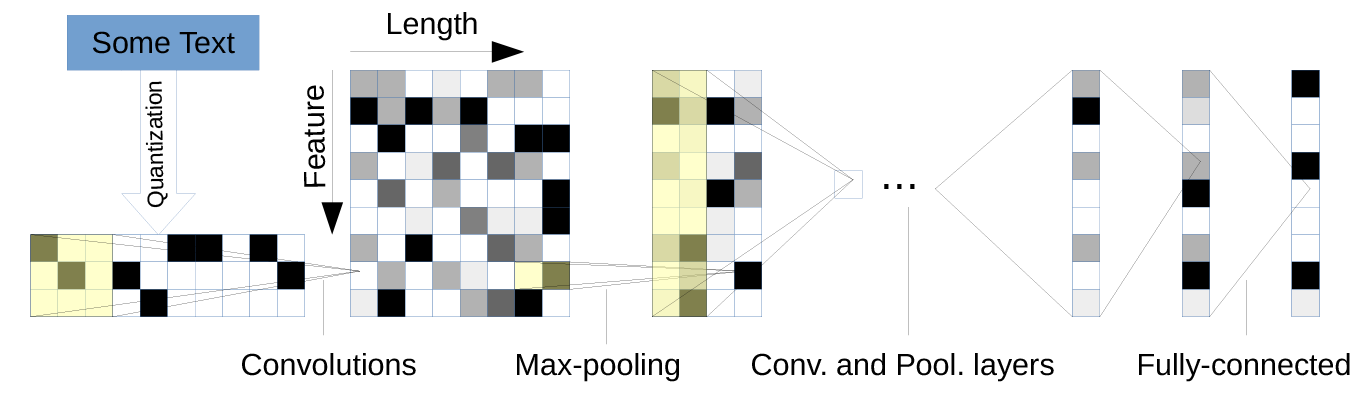
\includegraphics{char_cnn.png}
\end{figure}

The architecture of the Char-CNN is shown in Figure \ref{char_cnn}. The model receives the text and quantize each character. This pre-process is called character quantization which is done by prescribing an alphabet of size $m$ for the raw text, and each character is quantized into one-hot encoding. For English text, we normally use the alphabet consisting 70 characters, which is presented as follows
\begin{lstlisting}[language=Python]
  abcdefghijklmnopqrstuvwxyz0123456789
  -,;.!?:"/\|_@#$&*~`+-=<>()[]{}'^%
\end{lstlisting}
There are 26 English letters, 10 digits, 33 other characters and the new line character, which is not shown above. For example, the character ``b'' is quantized into [0,1,0,0,0,.....,0]. Only the second element has value of 1 while other elements are all zero. 

The encoded text is fed to the convolutional and the maxpooling layers after the quantization. These two layers are the key components of the ConvNets. In Char-CNN, the temporal, as known as one-dimensional, convolutional modules are used. The temporal convolution is similar to the convolutions commonly used in computer vision, which just simply computes a 1-D convolution. For a input function and a kernel function in form of $g(x)\in[1,l] \rightarrow \mathbb{R}$ and $f(x) \in [1,k] \rightarrow \mathbb{R}$, where $l$ is the input feature size and $k$ is the kernel size. The convolution function $h(y) \in [1, \frac{l-k}{d}+1] \rightarrow \mathbb{R}$ is defined as 
\begin{equation}
h(y) = \sum_{x=1}^{k} f(x) \cdot g(y \cdot d -x + c)
\end{equation}
where $d$ is the stride, $c$ is an offset constant which is defined as
\begin{equation}
c = k-d+1
\end{equation}
For a ConvNets with input feature size of $m$ and output feature size of $n$, each inputs and outputs element are $g_i(x)$ and $h_j(y)$ correspondingly. And the weight of the kernel is $f_{i,j}(x)$ where $i=1,2,...,m$ and $j=1,2,...,n$. The output $h_j(y)$ is the sum over $i$ of the convolutions between $g_i(x)$ and $f_{i,j}(x)$.	As objects tend to have a local spatial support, for example, the connect between each characters in a word, such computation can extract the local features which makes ConvNets so powerful.

After the convolutional layer, it is the temporal max-pooling layer which helps us to train deeper models. Pooling is a effective method used to combine several nearby features into a local global `bag of features' to preserve task-related information while removing irrelevant information. For example, the vector $\mathbf{v}$ with $P$ components is reduced by the pooling layer $h$ to a single scalar $h(v)$. There are two main pooling way: average pooling $h(\mathbf{v}) = \frac{1}{P} \sum_{i=1}^P v_i$ and max pooling $f(\mathbf{v}) = \mbox{max}_i v_i$. The temporal max-pooling is the same as spatial max-pooling except it is in 1-D~\cite{boureau2010theoretical}. For a input function $g(x)\in[1,l] \rightarrow \mathbb{R}$, the max-pooling function $h(y) \in [1, \frac{l-k}{d}+1] \rightarrow \mathbb{R}$ is defined as 
\begin{equation}
h(y) = \mbox{max}^{k}_{x=1} g(y\cdot d -x +c)
\end{equation}

In Char-CNN, there are 6 convoltional layers and the first two convolutional layers and the last convolutional layer followed by a max-pooling layer. The configurations of the convolutional layers are presented in Table \ref{config_char_cnn}

\begin{table}[]
\caption{The configurations of the convolutional layers in Character-level Convolutional Network}
\centering
\label{config_char_cnn}
\begin{tabular}{ccccc}
Layer & Feature & Kernel Size & Pooling Size &  \\ \cline{1-4}
1     & 1024    & 7           & 3            &  \\
2     & 1024    & 7           & 3            &  \\
3     & 1024    & 3           & N/A          &  \\
4     & 1024    & 3           & N/A          &  \\
5     & 1024    & 3           & N/A          &  \\
6     & 1024    & 3           & 3            & 
\end{tabular}
\end{table}

Following the 6 convolutional layers, there are 3 fully connected layers. The non-linearity used in Char-CNN is the ReLUs which defined as 
\begin{equation}
\mbox{ReLU}(x) = \mbox{max}(0,x)
\end{equation}
The configurations of the fully connected layers is shown in Table \ref{config_char_fl}
\begin{table}[]
\caption{The configurations of the fully-connected layers in Character-level Convolutional Network}
\centering
\label{config_char_fl}
\begin{tabular}{cc}
Layer & Output units      \\ \hline
7     & 1024              \\
8     & 1024              \\
9     & Number of classes
\end{tabular}
\end{table}

All the weights in the Char-CNN is initialed by a Gaussian distribution with mean of $0$ and standard deviation of $0.05$. Same as fastText, the Char-CNN is trained by stochastic gradient descent with batch size of 128. It also uses momentum to accelerate the descent. The 0.9 momentum is initialed with the step size of 0.01, which is halved 3 epochs for 10 times.

Compared with traditional machine learning method in text classification, such as bag-of-words~\cite{sparck1972statistical}, bag-of-ngrams, bag-of-means on word embedding~\cite{mikolov2013distributed}, and some deep learning methods, such as word-level ConvNets, Long-short term memory, Character-level Convolutional Network is an effective method and it performs better than most of the traditional machine learning methods in large datasets~\cite{zhang2015character}.

\subsection{Bidirectional Long-short Term Memory Network}
\begin{figure}
\centering
\caption{The mechanism of the recurrent neural network~\cite{Greff2017}}
\label{rnn}
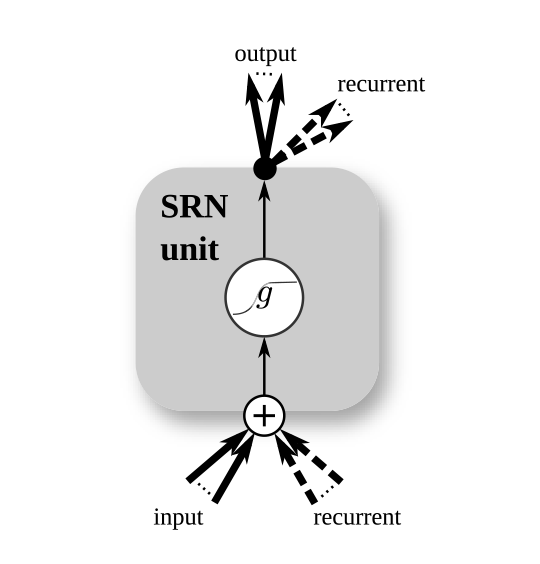
\includegraphics{rnn.png}
\end{figure}
Recurrent Neural Network (RNN) is treated as a good type of neural network to deal with sequence-like data, because it can use its internal state to process sequences of inputs and present the dynamic temporal behavior for the sequence. The basic mechanism of RNN is shown in Figure \ref{rnn}. The simplest form of RNN is an multiple layer perceptron with the previous set of the hidden unit activations feeding back into the network along with the inputs~\cite{bullinaria2013recurrent}. 

However, RNN has the gradient vanishing problem which makes it hard to train. To overcome this problem, many new types of recurrent neural networks were introduced. The Long-Short Term (LSTM) unit is one of the most effective units which was firstly proposed by Hochreiter and Schmidhuber~\cite{hochreiter1997long}. The basic idea behind LSTM units is that it introduces some gates to control the degree which the units keep the previous states and memorize the current inputs. The detailed schematic of LSTM unit is shown in Figure \ref{lstm}.
\begin{figure}
\centering
\caption{The schematic of the LSTM unit~\cite{Greff2017}}
\label{lstm}
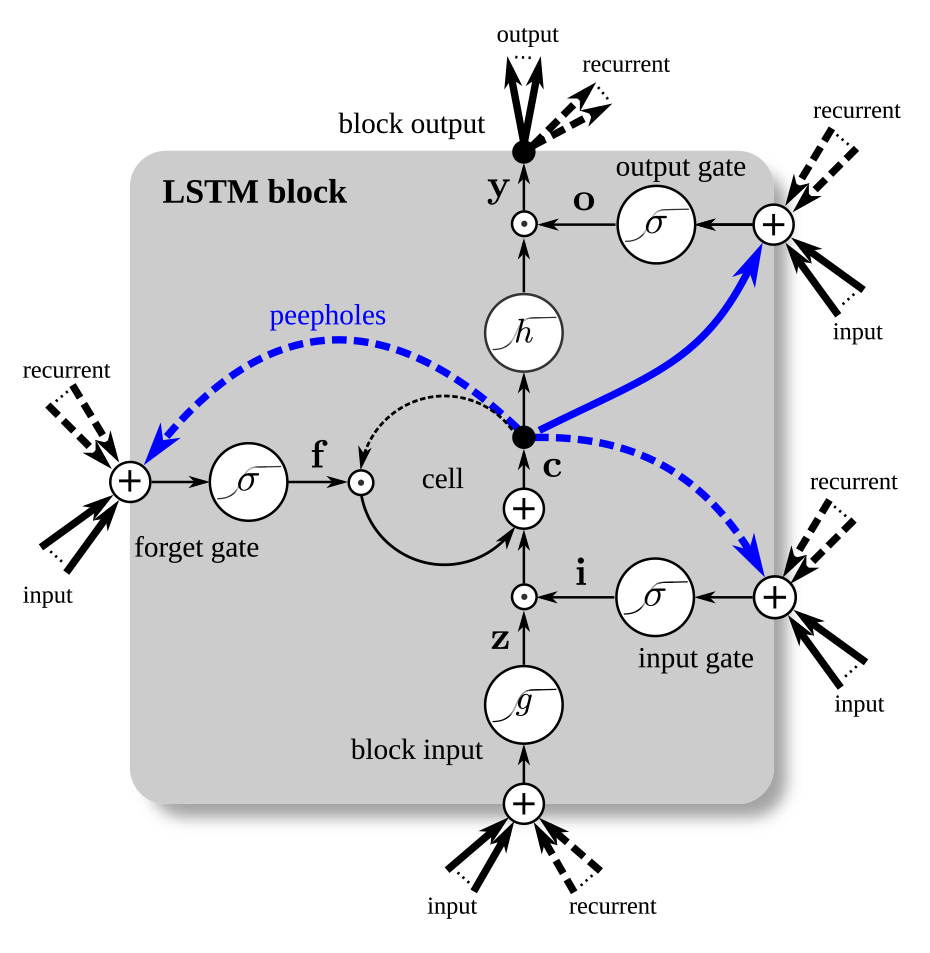
\includegraphics{lstm.png}
\end{figure}

We suppose the input vector at time $t$ is $\mathbf{x}^t$, the state at time $t-1$ is $\mathbf{h}^{t-1}$ $N$ is the number of LSTM units, and $M$ is the number of instances. There are following weights for the LSTM unit:
\begin{itemize}
	\item Input weights: $\mathbf{W}_z, \mathbf{W}_i, \mathbf{W}_f, \mathbf{W}_o \in \mathbb{R} ^{N\times M} $
	\item Recurrent weights: $\mathbf{R}_z, \mathbf{R}_i, \mathbf{R}_f, \mathbf{R}_o \in \mathbb{R}^{N\times N}$
	\item Peephole weights: $\mathbf{p}_i, \mathbf{p}_f, \mathbf{p}_o \in \mathbb{R}^{N}$
	\item Bias weights: $\mathbf{b}_z,\mathbf{b}_i, \mathbf{b}_f, \mathbf{b}_o \in \mathbf{R}^{N} $
\end{itemize}

Then the computation of LSTM layer forward propagation can be presented as
\begin{equation}
\mathbf{z}^t = g( \mathbf{W}_z \mathbf{x}^t + \mathbf{R}_z \mathbf{h}^{t-1} + \mathbf{b}_z)
\end{equation}
\begin{equation}
\mathbf{i}^t = \sigma( \mathbf{W}_i \mathbf{x}^t + \mathbf{R}_i \mathbf{h}^{t-1} + \mathbf{p_i} \odot \mathbf{c}^{t-1} + \mathbf{b}_i)
\end{equation}
\begin{equation}
\mathbf{f}^t = \sigma( \mathbf{W}_f \mathbf{x}^t + \mathbf{R}_f \mathbf{h}^{t-1} + \mathbf{p_f} \odot \mathbf{c}^{t-1} + \mathbf{b}_f)
\end{equation}
\begin{equation}
\mathbf{c}^t = \mathbf{z}^t \odot \mathbf{i}^t + \mathbf{c}^{t-1} \odot \mathbf{f}^t
\end{equation}
\begin{equation}
\mathbf{o}^t = \sigma( \mathbf{W}_o \mathbf{x}^t + \mathbf{R}_o \mathbf{h}^{t-1} + \mathbf{p_o} \odot \mathbf{c}^{t} + \mathbf{b}_o)
\end{equation}
\begin{equation}
\mathbf{h}^t = h(\mathbf{c}^t) \odot \mathbf{o}^t
\end{equation}
where $\sigma$, $g$, and $h$ are activation functions
\begin{equation}
\mbox{Logistic sigmoid: } \sigma (x) = \frac{1}{1+e^{-x}}
\end{equation}
\begin{equation}
\mbox{Hyperbolic tangent: } g (x) = h(x) = \mbox{tanh}(x)
\end{equation}
Based on this mechanism, LSTMs do not suffer from the optimization problem and can capture long-term temporal dependences. LSTMs have been applied to many difficult problem, such as handwriting generation~\cite{Graves2013}, translation~\cite{Luong2014}, speech synthesis~\cite{fan2014tts}. 

However, the disadvantage of LSTMs is that they ignore the future context as it only read the data in temporal order. To overcome this limit, Bidirectional LSTMs (BLSTM) introduces a second layer where the LSTM units process the sequence in opposite order. Based on this design, the model has the ability to extract the features both from past and future. There are two main method to combine the outputs from forward and backward propagation. One is concatenating two output into a  new vector at each time-step. Another way is using element-wise sum operator. In this case, the output at time $i$ is defined as 
\begin{equation}
\label{element_wise_sum}
\mathbf{h}^{t} = \mathbf{h}^{t,\leftarrow} \oplus \mathbf{h}^{t, \rightarrow}
\end{equation}

Zhang et al. firstly proposed a text classification model based on BLSTM~\cite{zhang2015relation}. The architecture of the model is shown in Figure \ref{blstm}. Similar to fastText model, the first layer is the embedding layer on word level. To use the knowledge of general domains, the weights of the embedding layer are initialized by the pre-trained word vector. The pre-trained word vector is obtained by the word2vector tool~\cite{Mikolov2013}. In the BLSTM layer, the output is obtained by sum the backward and forward outputs as introduced in Equation \ref{element_wise_sum}. Based on the hypothesis that only several key words and the associated features contribute to the classification, the model uses the max-pooling rather than average-pooling after the BLSTM layer to extract the semantic meaning of a sentence.
\begin{figure}
\caption{Model structure of bidirectional LSTM}
\label{blstm}
\centering
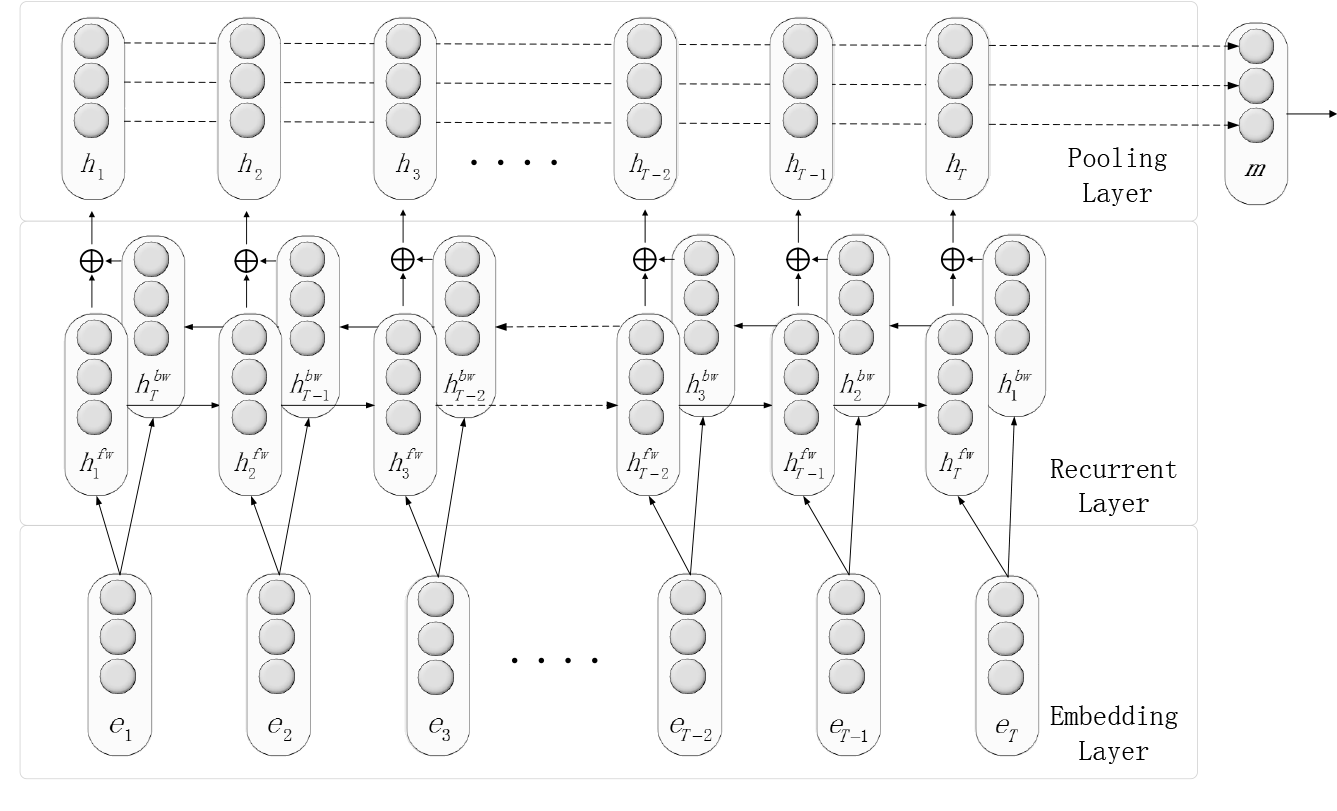
\includegraphics{blstm.png}
\end{figure}

The prediction result is given by the output layer with the activation function of softmax. Similar to aforementioned models, the loss function is the negative log-likelihood and the optimization is done by the stochastic gradient descent algorithm. In order to help propagating the gradient back to early steps easier, the fan-in technique is used to initialized the weights~\cite{plaut1987learning}. 





\subsection{Attention Based Bidirectional Long Short-Term Memory Network1}
Though, BLSTMs are effective models in dealing with sequence, it still has some disadvantages. As not every word in the sequence has the same importance, BLSTMs do not have such ability to capture the most important semantic information in a sentence. The ideal classification model is expected to be able to automatically focus on the words that have decisive effective on the prediction results. Attention mechanism was proposed to tackle this problem. Combining BLSTM and attention mechanism, a attention-based BILSTM (Att-BLSTM) for classification was proposed and outperforms most of the existing approaches~\cite{zhou2016attention}. The structure of A-BLSTM is shown in Figure \ref{attention_blstm}. In this model, the forward and backward is combined by the element-wise sum. 

Firstly, we suppose $\mathbf{H}$ is the matrix which consists the output vectors $[\mathbf{h}_1, \mathbf{j}_2,...,\mathbf{h}_T]$from BLSTM, where $T$ is the length of the sentence. The representation $\mathbf{r}$ of the sentence is defined as 
\begin{equation}
\mathbf{M} = \mbox{tanh}(\mathbf{H})
\end{equation}
\begin{equation}
\mathbf{\alpha} = \mbox{softmax}(\mathbf{w}^{\intercal}\mathbf{M})
\end{equation}
\begin{equation}
\mathbf{r} = \mathbf{H} \mathbf{\alpha} ^\intercal
\end{equation}
where $\mathbf{H} \in \mathbb{R}^{d\times T}$, $d$ is the dimension of the word vector. The sentence-pair representation used for linear classification is in form of
\begin{equation}
\mathbf{y}^* = \mbox{tanh}(\mathbf{r})
\end{equation}

\begin{figure}
\caption{Model structure of attention-based bidirectional LSTM}
\label{attention_blstm}
\centering
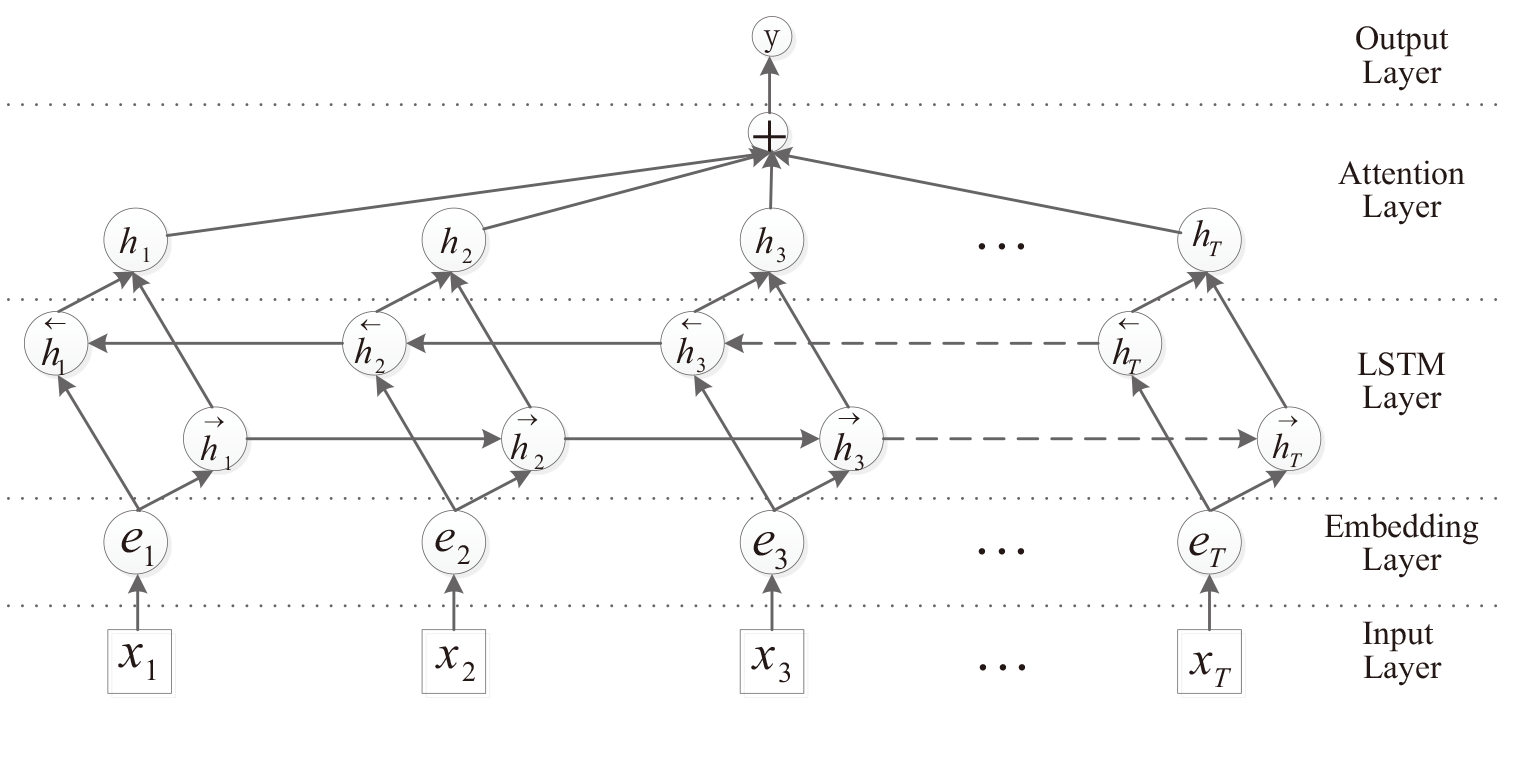
\includegraphics{attention_blstm.png}
\end{figure}

To avoid overfitting, A-BLSTM uses the nagative log-likelihood with L2 regularization:
\begin{equation}
L(\theta) = - \frac{1}{m} \sum_{i=1}^{m} t_i \mbox{log}(y_i) + \lambda \| \theta \|^2_F
\end{equation}
where $\mathbf{t}\in \mathbb{R}^m$ is the true label encoded as one-hot vector, $\mathbf{y}\in \mathbb{R}^m$ is the probability for each class produced by softmax function, $m$ is the number of classes, and $\lambda$ is the regularization hypeparameter which controls the penalty to the complex model.

In Att-BLSTM, dropout method is also used to do the regularization. During the training process, the dropout method is used on embedding layer and BLSTM layer. Dropout technique was first introduced by Hinton et al. in image classification\cite{krizhevsky2012imagenet}. It set the output of each neuron to zero with a specific probability. In this way, a part of neurons are dropped out and do not contribute to the forward and backward propagation. In Att-BLSTM, the dropout rate of embedding layer and LSTM layer is set as 0.3, 0.5 respectively.

The embedding layer is initialized by the pre-trained word embedding by Turian et al~\cite{turian2010word}. Other weights are initialized randomly. Different with aforementioned models which trained using stochastic gradient descent, Att-BLSTM is trained using AdaDelta~\cite{zeiler2012adadelta} with a learning rate of 1.0 and batch size of 10. The L2 regularization is set as $10^{-5}$.

Att-BLSTM achieve a similar result to the BLSTM which used many features derived from NLP tools and lexical resources~\cite{Zhang2015}. 




\chapter{Concept Drift Detection}
\label{exp1}
\section{Data Used}

The whole dataset was collected by web crawler, containing 181903 fashion news in www.hypebeast.com from 20/04/2005 to 13/06/2018. A sample of the dataset including the date of the publication, the category, the keywords, the title, the context, the HYPES, and the class of the HYPES. The HYPES is the real time popularity metric informing reader of what is trending. The HYPES is computed based on the page-viewers, the comments, and the information flow on social network. The HYPES is classified into 3 classes which is shown in Table \ref{popularityclasses} of the introduction chapter. 

During the development of the website, HYPEBEAST also changed the algorithm of computing the HYPES. Figure \ref{hypes_yeas} shows the change of the HYPES from 2015 to 2018. And the distribution of each class over the past 13 years is presented in Figure \ref{proportion_yeas}. It is obvious that after the middle of 2013, HYPES have a significant jump and the present a rising trend until 2018. However, the proportions of classes remain stable after 2014. Based on this intuitive analysis, we select the data from 01/01/2014 to 13/08/2018 as the dataset for the experiment. It containing 95787 fashion news. The distribution of the classes is shown in Table \ref{distribution_classes}

\begin{figure}
\centering
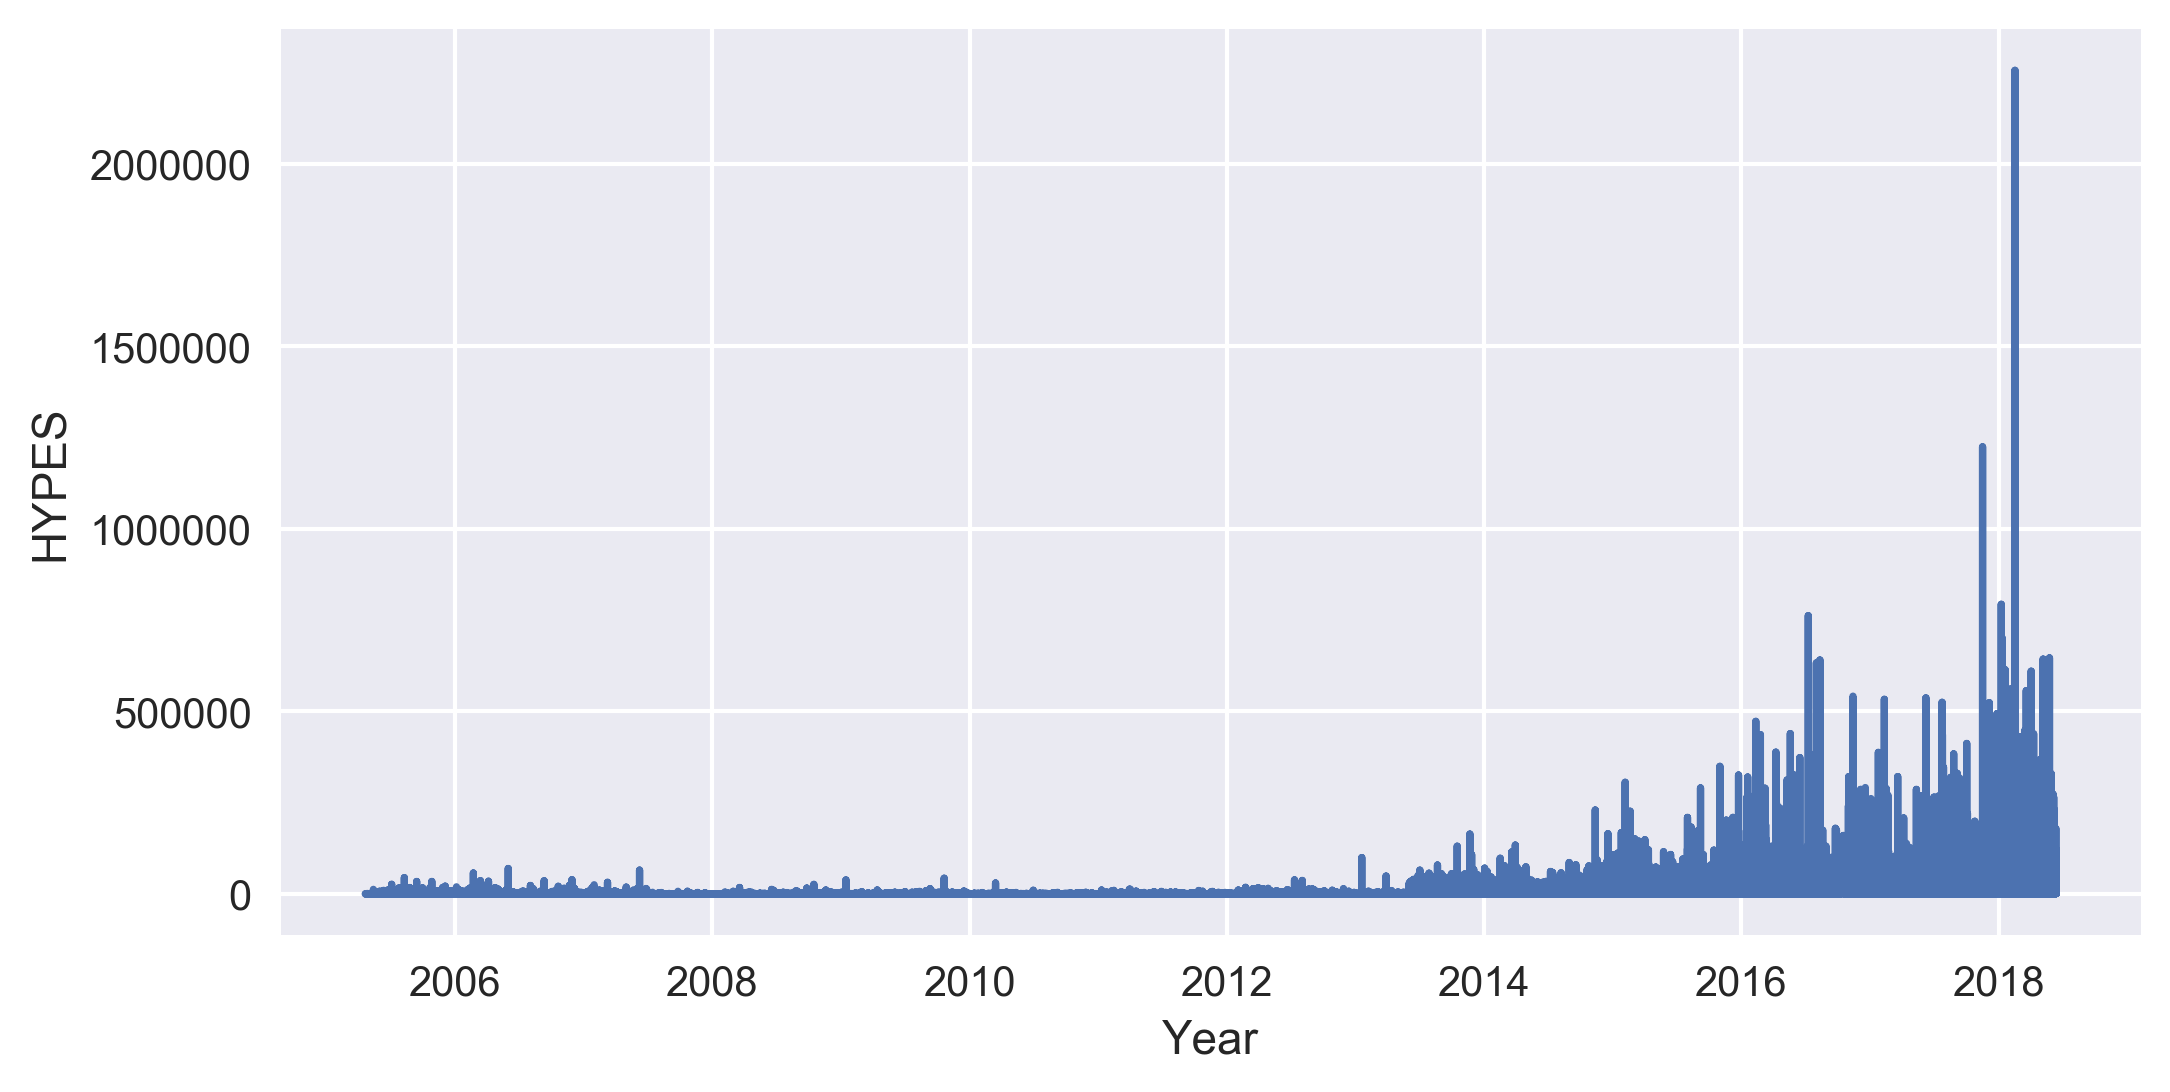
\includegraphics[width=0.9\textwidth]{hypes_year.png}
\caption{HYPES over years}
\label{hypes_yeas}

\end{figure}

\begin{figure}
\centering
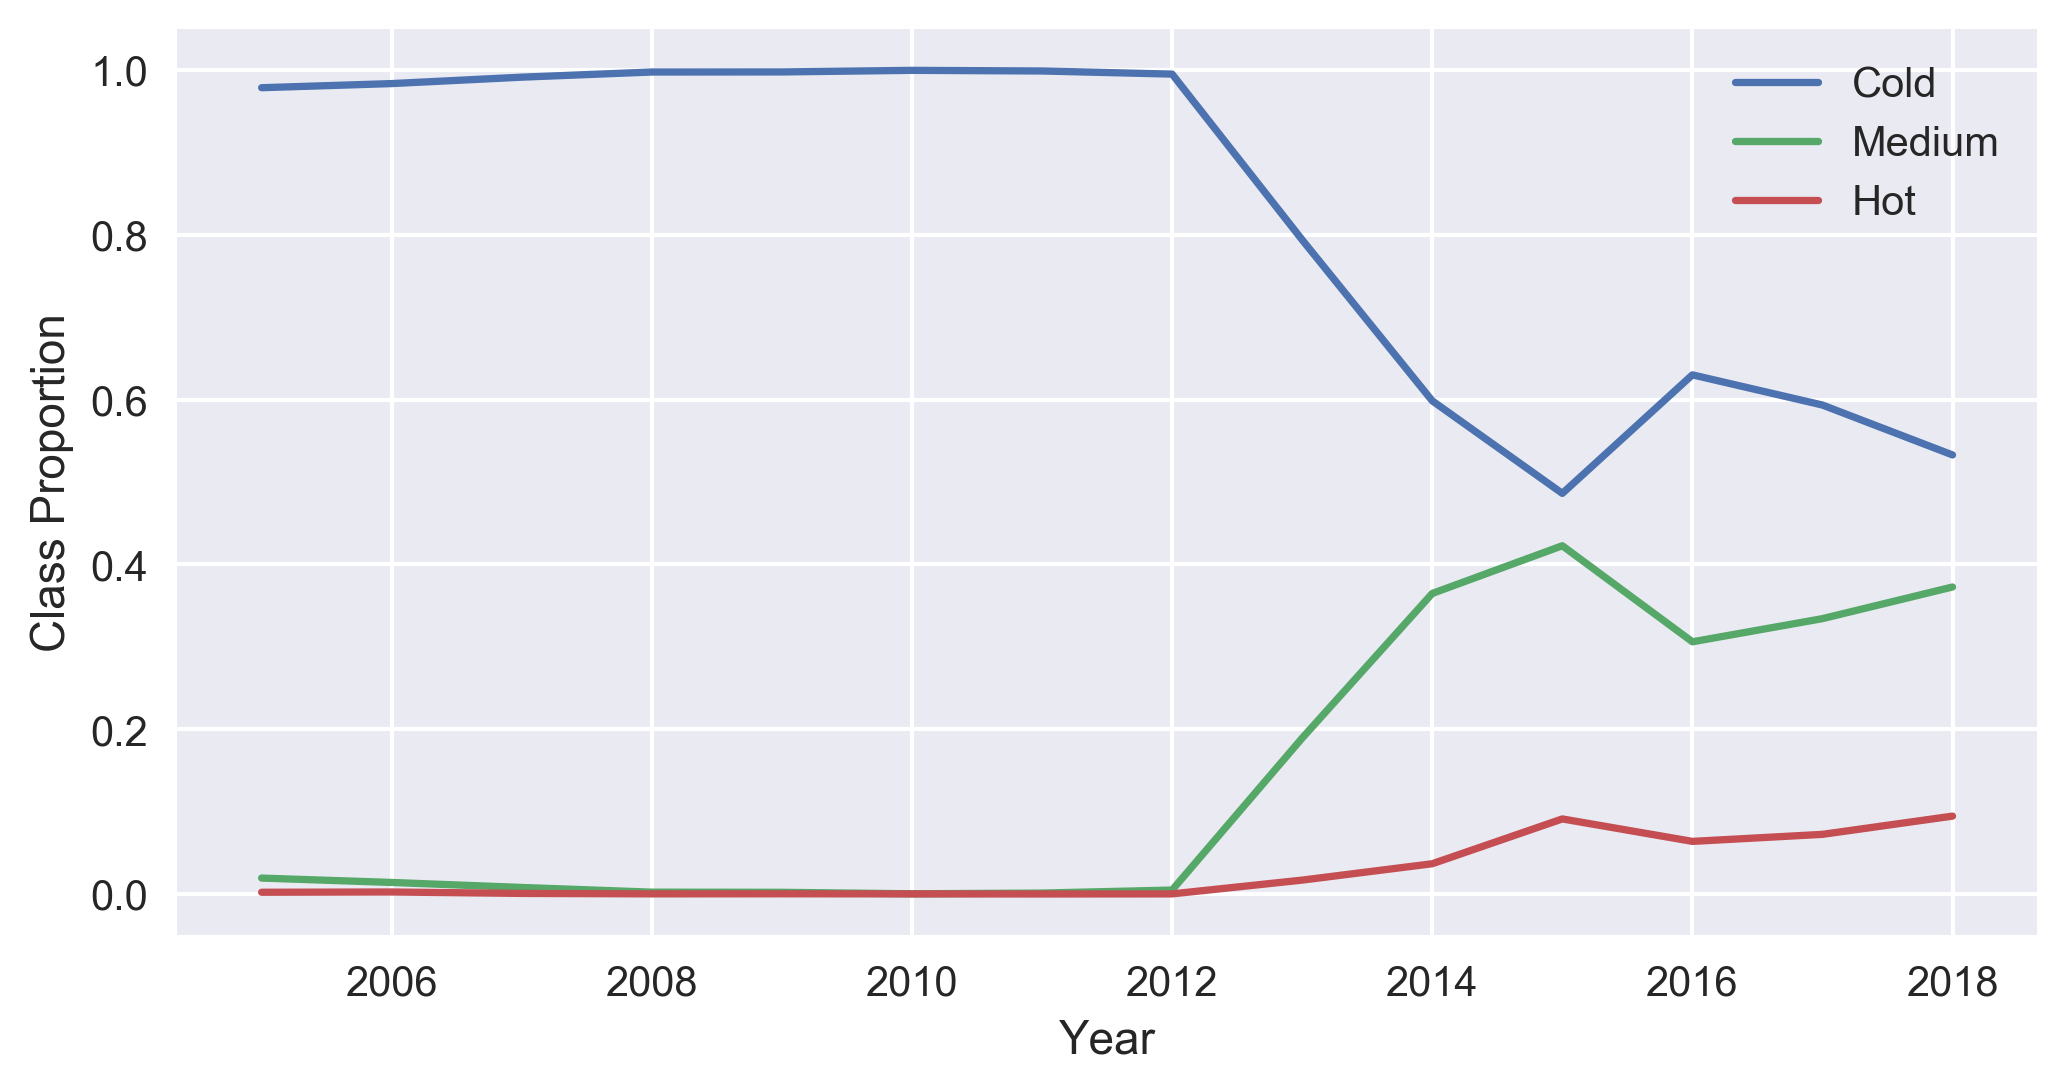
\includegraphics[width=0.9\textwidth]{proportion_hypes.png}
\caption{Proportion of each class over years}
\label{proportion_yeas}
\end{figure}


\begin{table}[]
\centering
\begin{tabular}{lll}
\multicolumn{1}{c}{Popularity} & \multicolumn{1}{c}{Number} & Proportion \\ \hline
Cold                           & 52852                      & 0.5518     \\
Meidum                         & 35944                      & 0.3752     \\
Hot                            & 6991                       & 0.0730    
\end{tabular}
\caption{Distribution of classes of the dataset}
\label{distribution_classes}
\end{table}




\section{Model Design}
As shown in Figure UNKNOWN, the model proposed in this experiment contains three components: (1) a pre-process part that extract features from raw text; (2) a base learner that gives a prediction with a subset of examples; (3) a concept drift detection algorithm which detects the drift and select the subset of the example to re-train the base learner. These components will be presented in detail in this section.

\subsection{Preprocessing}
Before the training data can be fed to the model, it needs to be transformed to a format the model can understand which is called preprocessing including tokenization, vectorization, and feature selection. The scheme of the pre-processing is shown in Figure UNKNOWN.

In natural language processing problem, tokenization is the procedure of splitting a text into words, phrases, or other meaningful parts. In the other words, tokenization is kind of segmentation. In conventional machine learning problem, Bag-of-words model is the most popular representation to tokenize the text. In this model, a raw article is represented as a bag of its words. It is a commonly used and also very effective model. However, bag-of-words model ignores the order of the words which leads to the same representations of the sentences ``Kanye loves Kim.'' and ``Kim loves Kanye.''. As an alternative, the bag-of-ngam model is used to store the spatial information. To some extent, bag-of-words is a special type of bag-of-ngram which only counts the unigram. 

For example, in a bag-of-ngrams model, text is represent as a collection of unique ngrams (groups of $n$ adjacent tokens). Consider the text ``The YEEZY BOOST restock gets postponed''. Here, the word unigrams $(n=1)$ are ['The', `YEEZY', `BOOST', `restock', `gets', `postponed'] and the bag-of-bigrams $(n=2)$ is ['The YEEZY', `YEEZY BOOST', `BOOST restock', `restock gets', `gets postponed']. 

In this experiment, we tokenize the text into both unigrams and bigrams which not only consider the distribution of the words but also the local connection between the words. Thus, the tokenization result of the sentence aforementioned is 
\begin{lstlisting}[language=Tex,basicstyle = \ttfamily, breaklines = true]
['The', `YEEZY', `BOOST', `restock', `gets', `postponed', 'The YEEZY', `YEEZY BOOST', `BOOST restock', `restock gets', `gets postponed']
\end{lstlisting}

After the tokenization,the ngrams need to be truned into numerical vectors which can be processed by the machine learning algorithm. Firstly, every ngram is assigned a unique index which ranges from 0 to the number of ngrams in the corpus. The example below shows the indexes assigned to the unigrams and bigrams generated for two sentences.

\begin{lstlisting}[language=Tex,basicstyle = \ttfamily, breaklines = true]
Raw texts: 
	`Where to buy the YEEZY BOOST.'
	`Your first look at the YEEZY BOOST.'
Index assigned for every ngrams: 
	{'Where': 7, `to': 6, `buy': 2, `the': 5, `YEEZY': 8, `BOOST': 1, `You': 9, `first': 3, `look': 4, `at': 0}
\end{lstlisting}

Once the indexes are siggned to the ngrams, we vectorize using the encoding methods. There are three popular encoding methods. The first one is the one-hot coding by which the text is represented as a vector indicating the presence or absence of a token in the text. The second one is the count encoding by which the text is encodded as a vector indicating the count of a ngrams. The disadvantage of the above two methods is that common words such as `the', `and' are not pernalized. These words occurs in similar frequencies in all texts and are not particularly unique to the text samples in the dataset. Thus, in our model, we use the tf-idf encoding to represent the ngrams. $\mbox{tf}$ means term frequency and $\mbox{idf}$ means inverse document frequencey. The formula used to compute the tf-idf of ngrams is that
\begin{equation}
\mbox{tf-idf}(d,t) = \mbox{tf} * \mbox{idf}(d,t)
\end{equation}
and the $\mbox{idf}$ is computed as 
\begin{equation}
\mbox{idf}(d,t) = \mbox{log} (\frac{n}{\mbox{df}(d,t)}) +1
\end{equation}
where $n$ is the total number of documents and $\mbox{df}(d,t)$ is the document frequency which is defined as the number of documents $d$ that contain term $t$. The constant `$1$' is added to make the terms with zero $\mbox{idf}$ will not be entirely ignored. tf-idf helps to ajust for the fact that some words appear more frequently in general.

During above process, we also apply some tricks. One of them is the lowercase conversion. Since uppercase or lowercase forms words are assumed to have no difference. Another is the stop-words removal. The stop-words are usually assumed to be irrelevant in text classification~\cite{uysal2014impact}.

The vectorized feature vectors are alway high-dimensional in text classification problem because the size of the corpus is very large. In addition, not every feature extracted from the text is useful for the classification. In this case, feature selection is a necessary step which is helpful (1) to improve the performance of the classifier and avoid the overfitting; (2) to reduce the memory storage and provide a more cost-effective model (3) to gain a deeper insight into the underlying processes that generated the data. 

If the features are categorical, we normally calculate a chi-square statistic between each feature and the target vector. However, the encoded features are quantitative. Therefore, we select the features by computing the ANOVA F-value between each feature and the target vector. The F-val scores examine if, when we group the numerical features by the target vectors, the means for each group are significantly different. Based on F-val scores, we can remove the features so as are statistically uncorrelated with class labels.

Suppose the encoded feature vectors $\mathbf{X} \in \mathbb{R}^{n\times m}$, where $n$ is the number of examples and $m$ is the number of features, and the labels $\mathbf{Y} \in \mathbb{R}^{n\times l}$, where $l$ is the number of classes. We assume to select $k$ relevant features from $m$ features. Hence, there are $(n \choose k)$ combinations. Then, we compute the F-score for each combination with the ANOVA table and retain the $k$ features from the group with the highest F-score. 


\subsection{Base Learner}
In the experiment, the naive bayes classifier is used as base learner. It is because it naturally support incremental learning which can provide a fast and cost-efficient model.

For a given document $d$ with class of $y$, the Bayes' theorem present the relationship as a follow:
\begin{equation}
P(y|d) = \frac{P(d|y) p(y)}{P(d)}
\end{equation}
As what we mentioned in section of pre-processing, the document $d$ is represented as features $(x_1, x_2,...,x_k)$. The Naive Bayes method using a strong and naive assumption that the feature probabilities $P(x_i|y_j)$ are independent given the class $y$. Hence, the relationship is simplified to

\begin{equation}
\begin{aligned}
P(y|d) & = p(y|x_1,...,x_k) \\
	   & = \frac{P(y)P(x_1,..x_k|y}{P(x_1,..,x_k)}\\
	   & = \frac{P(y)\prod_{i=1}^kP(x_i|y)}{P(x_1,...,x_k)}\\
	   & \propto P(y)\prod_{i=1}^kP(x_i|y)
\end{aligned}
\end{equation}

The prediction result can be obtained by using the Maximum A Posteriori (MAP)
\begin{equation}
\hat{y} = \mbox{argmax}_y P(y)\prod_{i=1}^kP(x_i|y)
\end{equation}

In the experiment, we use the multinomial naive Bayes algorithm which is commonly used in text classification. The data distribution is parametrized by the vectors $\mathbf{\theta}_y = (\theta_{y_1}, ..., \theta_{y_k})$ for each class $y$, where $\theta_{y_i}$ is the probability $P(x_i|y)$ which is estimated as

\begin{equation}
\hat{\theta}_{y_i} = \frac{N_{y_i} + \alpha}{N_y+\alpha k}
\end{equation}

where $N_{y_i}$ is the number of times feature $i$ appears in a sample of class $y$ in the training set and $N_y$ is the total count of all features for class $y$.

The hypeparameter $\alpha$ is the smoothing parameter which incorporate a small-sample correction. It is a type of regularization. When a given test point whose class and one of features never occur together in the training set, the estimated probability will be zero. Because of the multiplication, the posteriori will be zero. Thanks to the smoothing parameters, no probability is set to zero. When $\alpha=1$, the smoothing is called Laplace smoothing, and Lidstone smoothing in the general case.

\subsection{Concept Drift Detection Algorithm}

In the experiment, we use Drift Detection Method (DDM) proposed by Gama et al.~\cite{gama2004learning}. Previous experiments have prove that DMM has the best performance in both gradual and abrupt drift~\cite{Goncalves2014}. In addition, compared with other detector, DMM is relative fast and cost-efficient. 

DMM was proposed by the probably approximately correct learning model~\cite{michalski2013machine} that if the distribution of the data is stationary, the error rate of the classifier will decrease with the increase of the number of the instances. Therefore, a great increase of the error rate indicates the change of the distribution, namely, the concept drift. 

For every instance at time $i$, the error-rate $p_i$ and the standard deviation $s_i = \sqrt{p_i(1-p_i)}$ are computed. $p_{min}$ and $s_{min}$ are stored when $p_i$ and $s_i$ reach their minimum. A warning level is reached if $p_i + s_i \geq p_{min} + w \cdot s_{min} $ and a drift occurs when $p_i + s_i \geq p_{min} +d \cdot s_{min}$, where $w$ and $d$ are number of standard deviation to warn ($w$) and detect ($d$) drift. With confidence levels for warning and drift set to 95\% and 99\% respectively, $w$ is $2$ and $d$ is $3$. When a warning level is reached, the instances after the warning level are stored. Once the drift occurs, the base learner will re-trained by the stored instance and the values of $p_{min}$ and $s_{min}$ will be reset. It often happens that the error rate increases and reach the warning level but decrease later. It is called false alarm. Once the false alarm occurs, the stored instances will be thrown away. Based on this mechanism, DDN keeps the base learner better adapted to the present data distribution.

DMM can be applied to any machine learning algorithm. It can be directly implemented inside the incremental learning algorithm and also can be implemented as a wrapper to batch learner. In this experiment, the DMM is implemented as a wrapper over the multinomial Bayes classifier that incrementally learns the dataset. Figure UNKOWN presents the process at time $i$


\begin{algorithm}
\caption{DMM with Bayes Classifier}
\label{ddm}
\begin{algorithmic}
\Require $\Phi$: Current Bayes Classifier, $\mathbf{x}_i, y_i$: Current example
\State Let $\hat{y_i} \leftarrow \Phi(\mathbf{x}_i)$
\State Compute $p_i$ and $s_i$

\If{$p_i + s_i < p_{min} + s_{min} $}
	\State $p_min \leftarrow p_i$ 
\EndIf

\If{$p_i + s_i < p_{min} + w \cdot s_{min}$}
	\State Warning $\leftarrow$ False
	\State Update $\Phi$ with $\mathbf{x}_i, y_i$
\Else
	\If{$p_i + s_i < p_{min} + d \cdot s_{min}$}
		\If{Not Warning?}
			\State buffer $\leftarrow \{\mathbf{x_i}, y_i\}$
			\State Warning? $\leftarrow$ True
		\Else
			\State buffer $\leftarrow$ buffer $\cup \{\mathbf{x_i}, y_i\}$
		\EndIf
	\Else
		\State Retrain $\Phi$ with the instances in the buffer
		\State Warning? $\leftarrow$ False
		Reset $p_min$ and $s_min$
	\EndIf 
\EndIf 
%\STATE $s_min \leftarrow s_i$ 
%\ENDIF
\end{algorithmic}
\end{algorithm}

\subsection{Evaluation Step}
To evaluate the performance of the concept drift detector, we use an approach described by Elwell et al.~\cite{Elwell2011}. For each time $t$, the instance from time $t+1$ is used as the test data. We assume $T$ as the time step. For each time step $T$, there are specific amount of test instances. Then, a variety of metrics is computed for each time step to compared the performance between the concept drift detector and the base learner. 

Firstly, we focus on the basic metric, the accuracy. For each test instance, the Bayes Classifier will return a boolean value indicating if it correctly classified the instance or not. For every time step $T$, the accuracy is defined as

\begin{equation}
\mbox{Accuracy} = \frac{\mbox{Number of correctly predicted instance} }{\mbox{Number of instances}}
\end{equation}

However, the data set is imbalanced, the number of hot news is significantly less than other two types of news. High accuracy does not indicate good classification ability. Using accuracy to evaluate the models will drive the models focus on the majority class but ignore the minority. In this case, accuracy alone is typically not enough information to do the comparison. In addition, we expect the hot news can be predicted correctly as much as possible. Thus, the recall is used to check if the model returns most of the relevant result.

For binary classification, recall is intuitively defined as 
\begin{equation}
\mbox{Recall} = \frac{tp}{tp+fn}
\end{equation}
where $tp$ is the number of correctly predicted positive instances, and $fn$ is the predicted correctly negative instance. However, our model is designed to deal with multiclass classification problem. The definitions of true positive ($tf$) and false negative ($fn$) are slightly different. The multiclass problem is separated into several binary classification problem. For class $i$, the true positive $tf_i$ and false negative ($fn_i$) are computed by treating class $i$ as the positive class and other classes are all negative. Then, we compute the micro-average recall as it aggregates the contributions of all classes to compute the average metric. The micro-average recall is defined as~\cite{sokolova2009systematic} 
\begin{equation}
\mbox{micro-Recall} = \frac{\sum_i tp_i}{\sum_i(tp_i + fn_i)}
\end{equation}

In addition, we also compute the micro average F1 score which is the weighted average of micro-average precision and micro-average recall.

\begin{equation}
\mbox{micro-F}_1 = 2 * \frac{\mbox{micro-Precision} * \mbox{micro-Recall}}{\mbox{micro-Precision} + \mbox{micro-Recall}}
\end{equation}

where definition of the micro-average precision is similar to the micro-average recall which is shown as a follow
\begin{equation}
\mbox{micro-Precision} = \frac{\sum_i tf_i}{\sum_i(tf_i + fp_i)}
\end{equation}
where $fp$ is number of negative instances which are predicted as positive.

In addition to pay attention the prediction result of the instances at each time step, the overall performance of the model will be evaluated as well. Apart from accuracy, micro-average recall, and micro-average F1 score, the normalized confusion matrix will be computed and visualized.

\subsection{Parameters Configuration}
The base learner only has a parameter, the additive smoothing parameter, which needs to be tune. A 5-fold cross-validation is applied and $\alpha$ is set to $0.1$. In addition, based on 5-fold cross-validation, we keep the top $20000$ features as the input.

The DDM has three parameters, including the minimum number of instances before permitting detecting change ($n$), the number of standard deviations to warn ($w$) and detect ($d$) drift. Testing is performed using following values for the parameters: $n\in\{15,30\}$,$w\in\{1.5,2.0\}$, and $d\in\{2.5,3.0\}$. The detectors with different parameters are presented in Table \ref{para_config}


\begin{table}[]
\caption{Parameter configuration of the drift detectors}
\label{para_config}
\centering
\begin{tabular}{cccc}
Detector & $n$  & $w$   & $d$   \\ \hline
1        & 30 & 2.0 & 3   \\
2        & 30 & 1.5 & 2.5 \\
3        & 50 & 2.0 & 3.0 \\
4        & 50 & 1.5 & 2.5
\end{tabular}
\end{table}


\section{Experimental Results}

\begin{figure}
\centering
\subfigure[Accuracy]{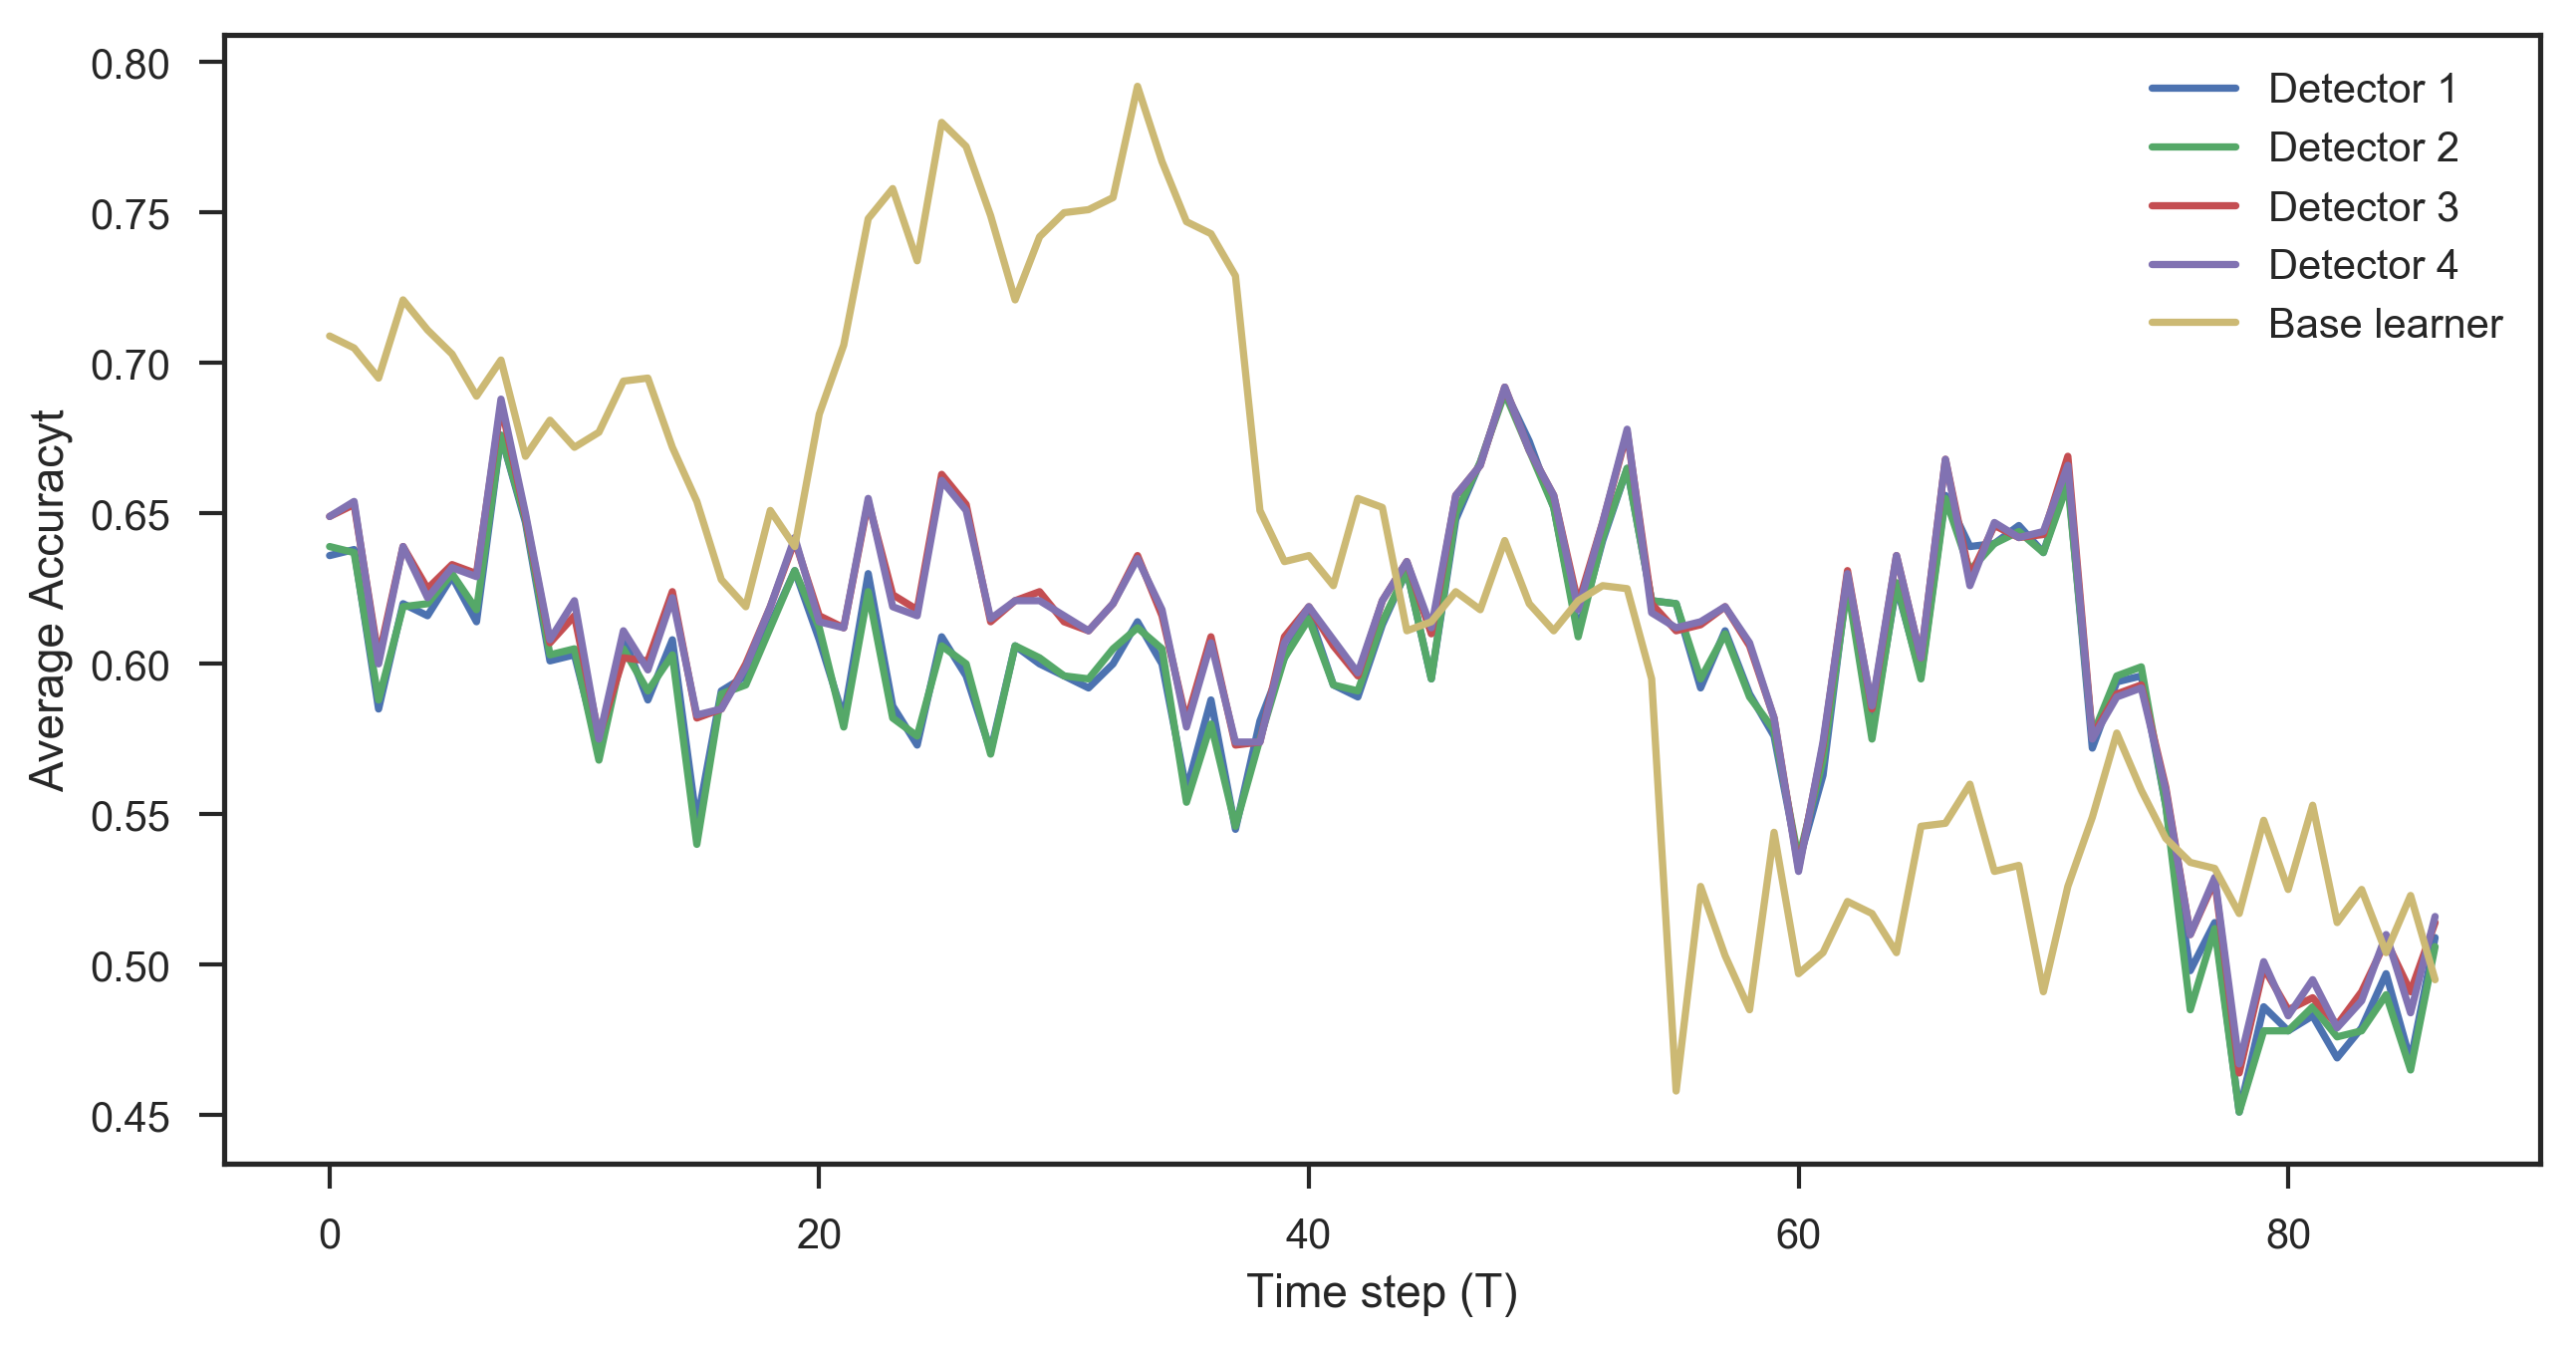
\includegraphics[width=0.9\textwidth]{drift_acc.png}}
\subfigure[macro-average Recall]{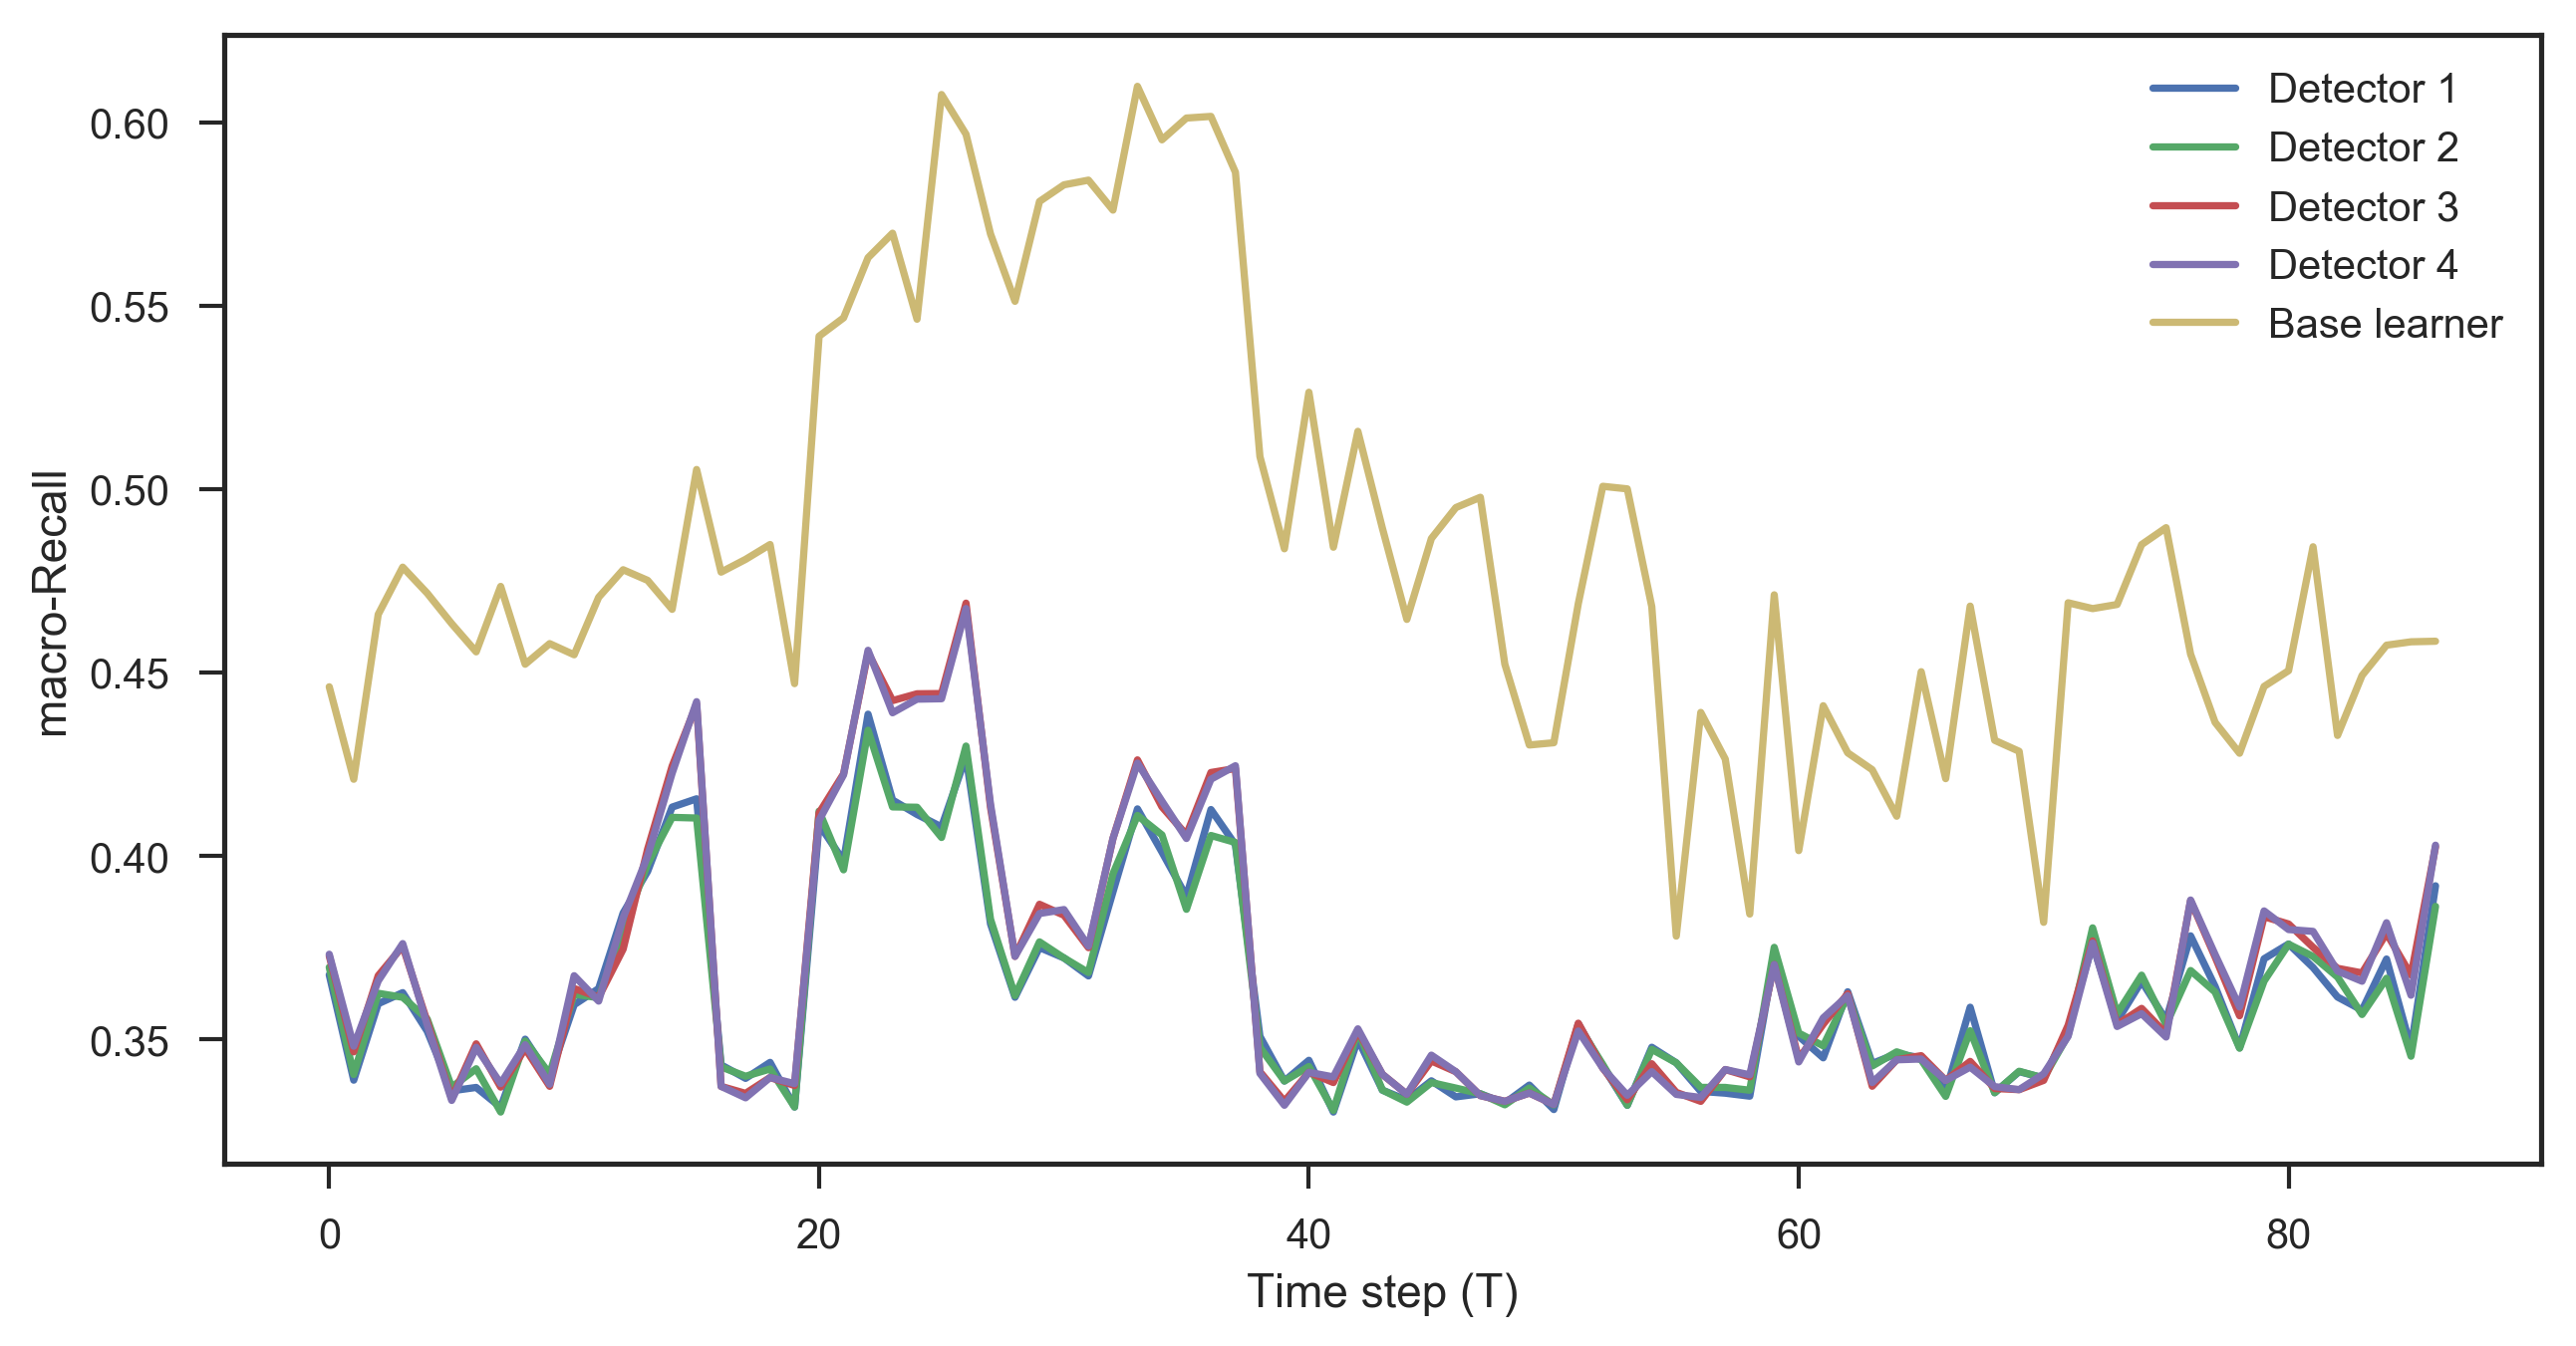
\includegraphics[width=0.9\textwidth]{drift_recall.png}}
\subfigure[macro-average F1 score]{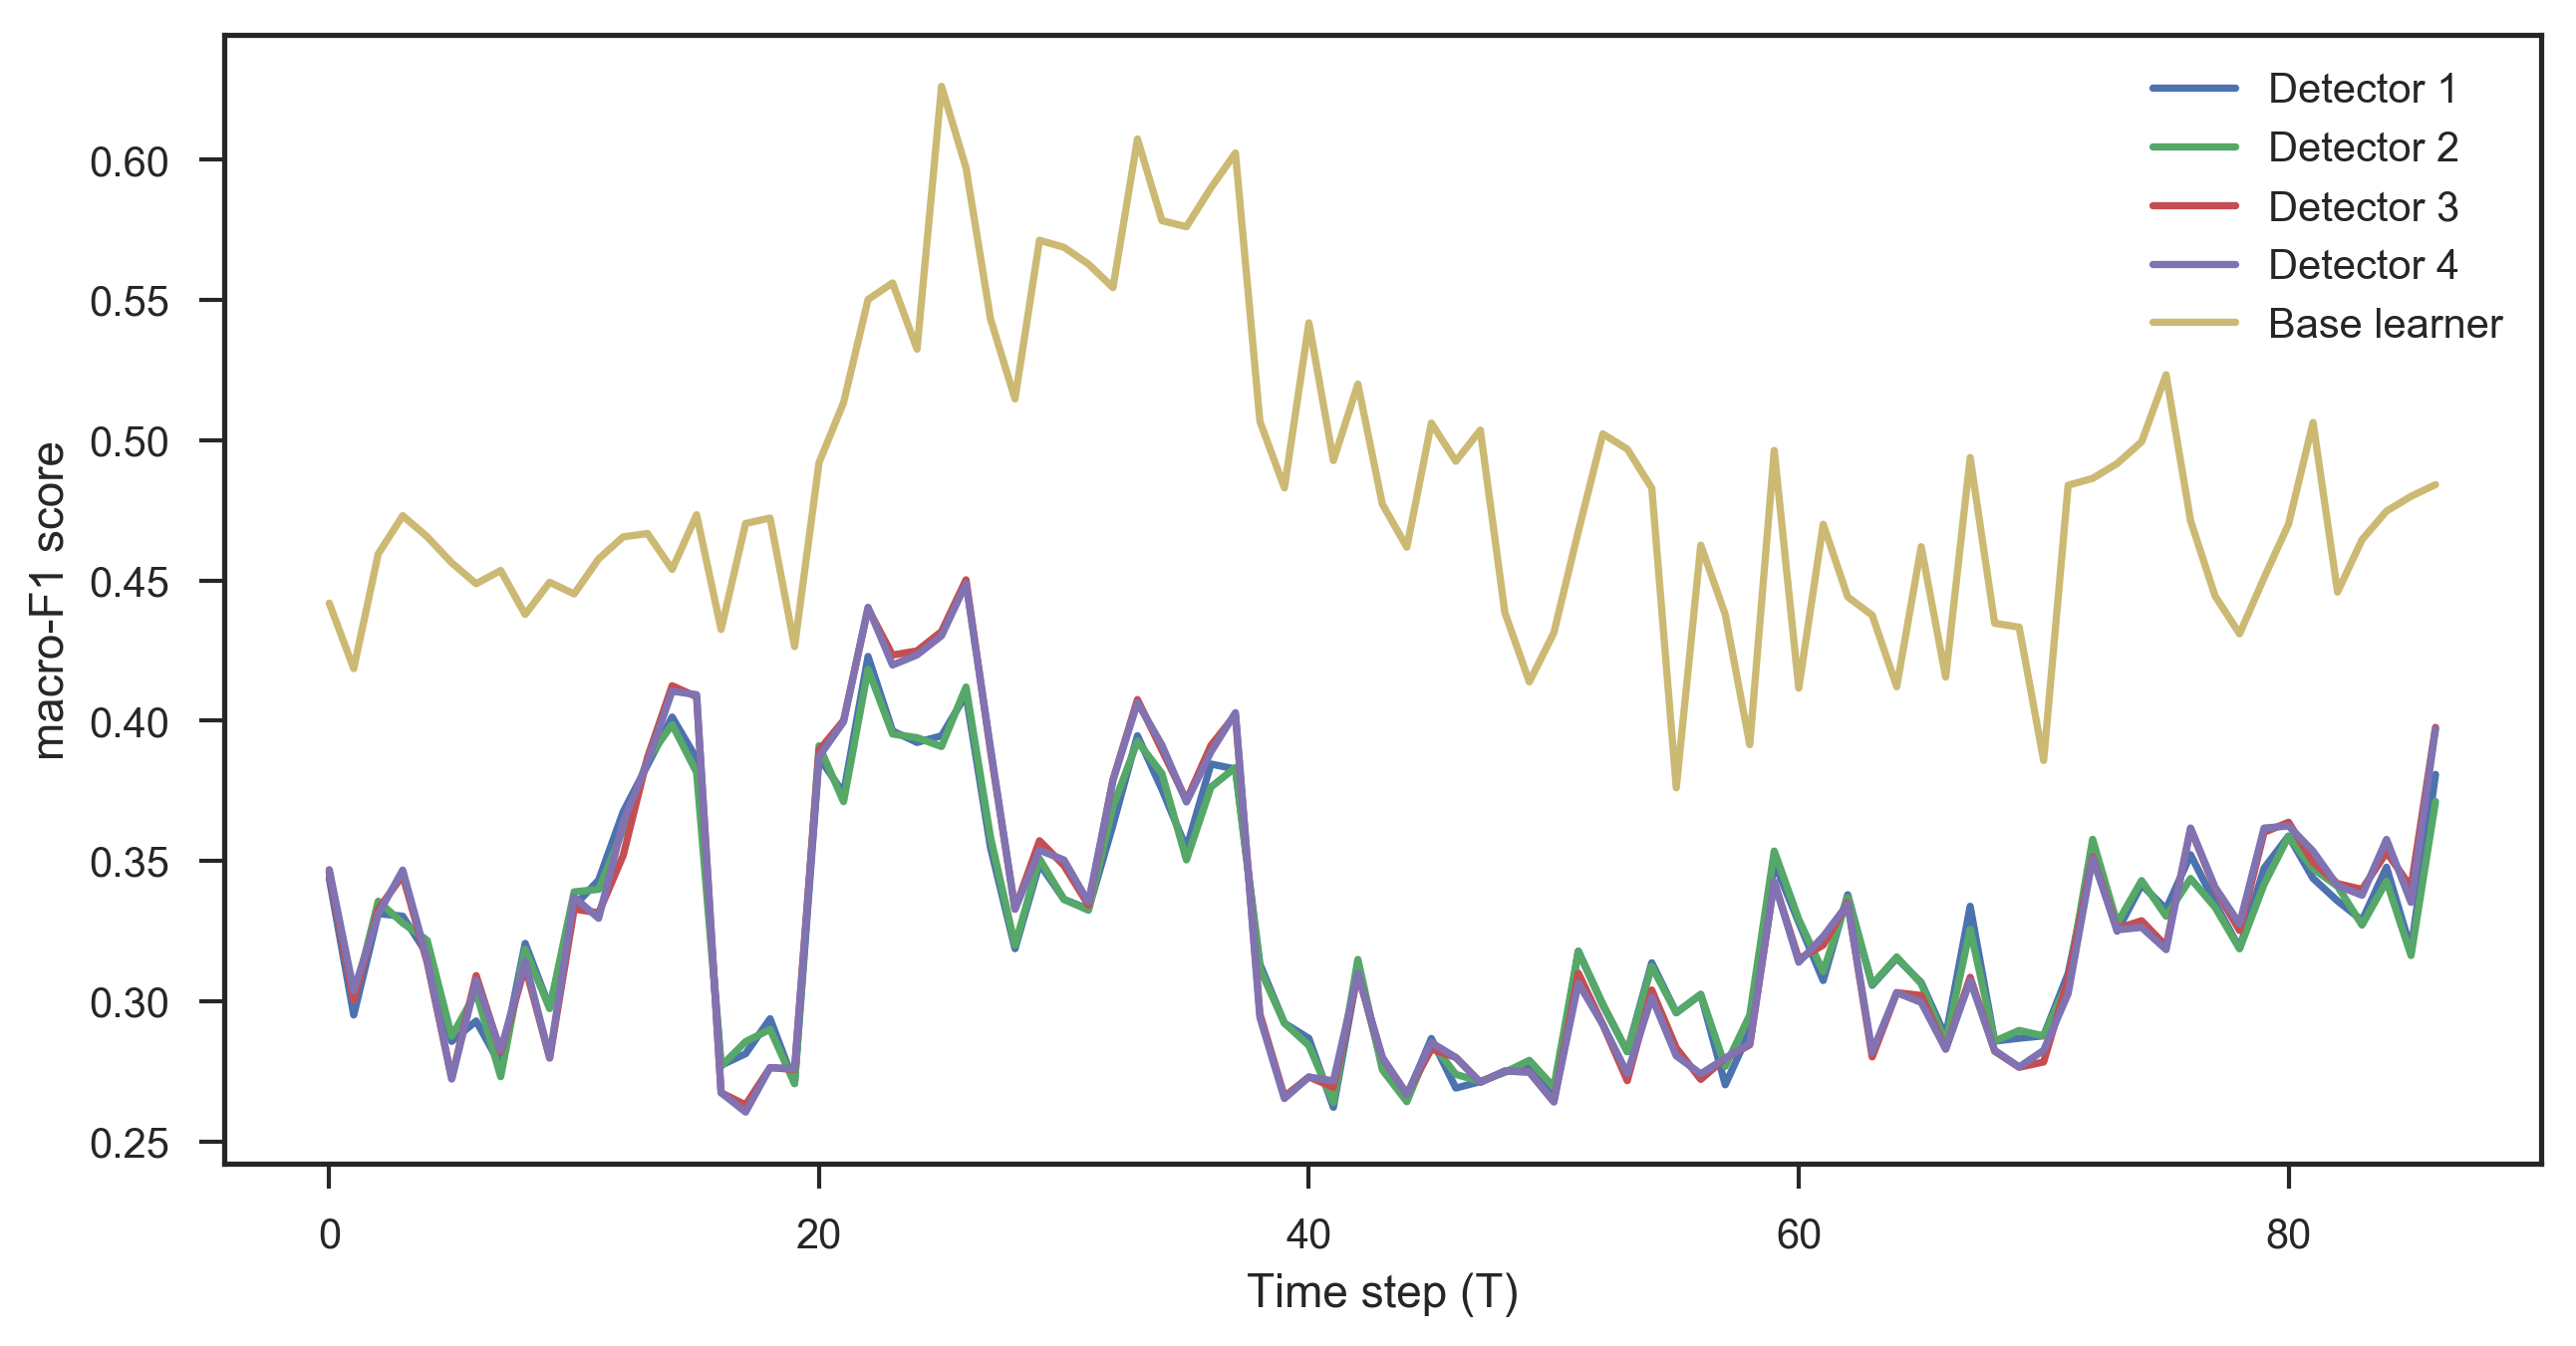
\includegraphics[width=0.9\textwidth]{drift_f1.png}}
\caption{Metrics of the detectors with different parameters.}
\label{drift_metrics}
\end{figure}

\begin{figure}
\centering
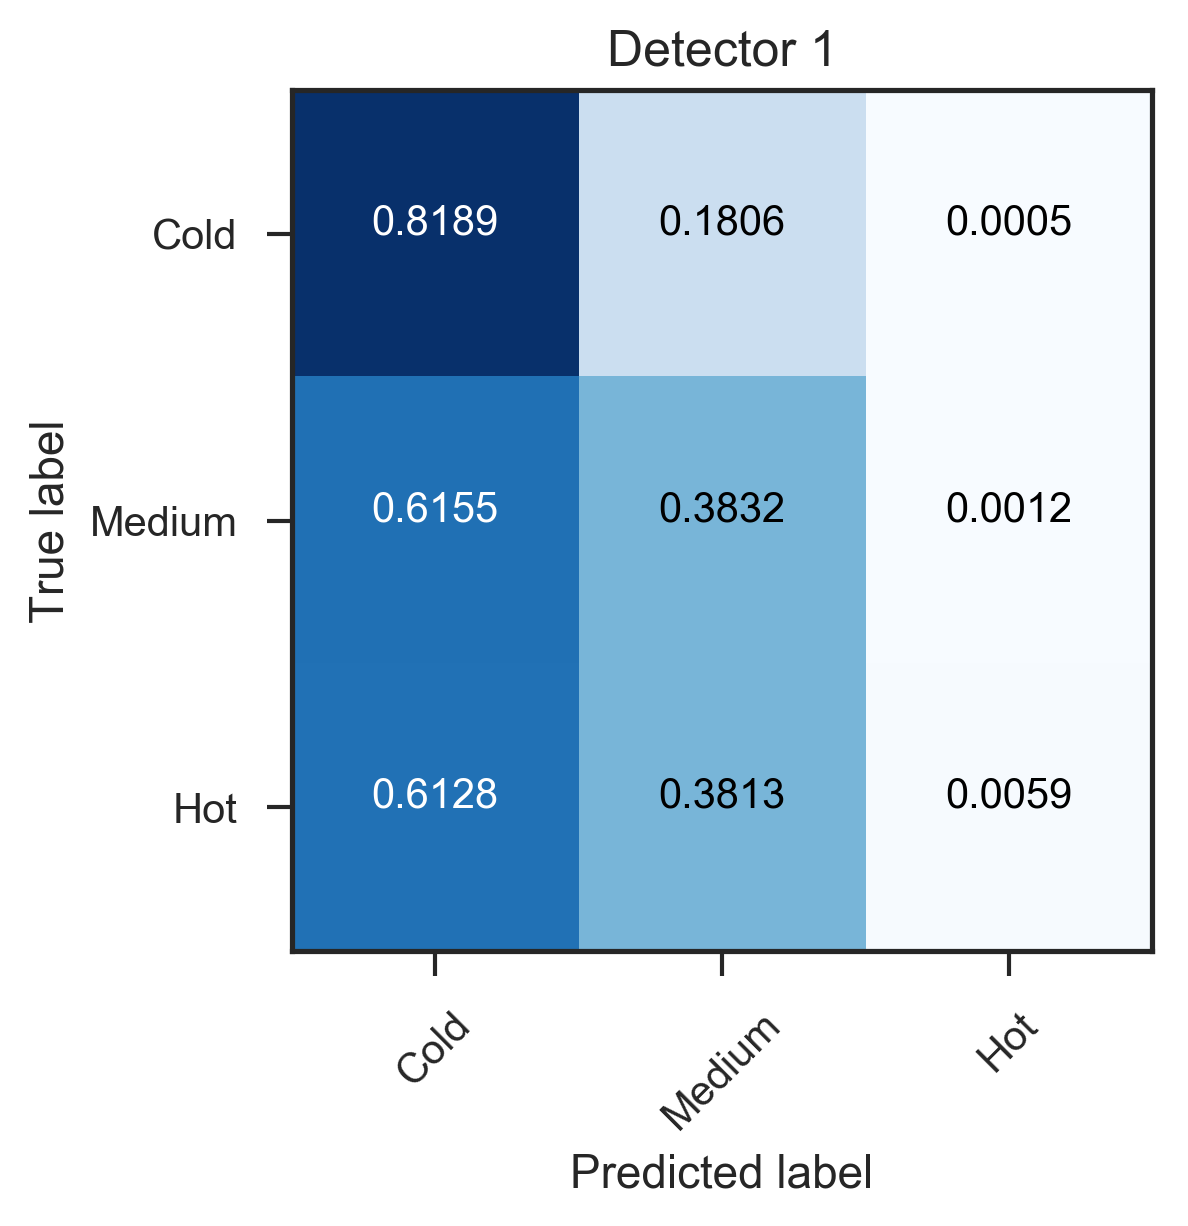
\includegraphics[width=0.45\textwidth]{drift_cm_Detector1.png}
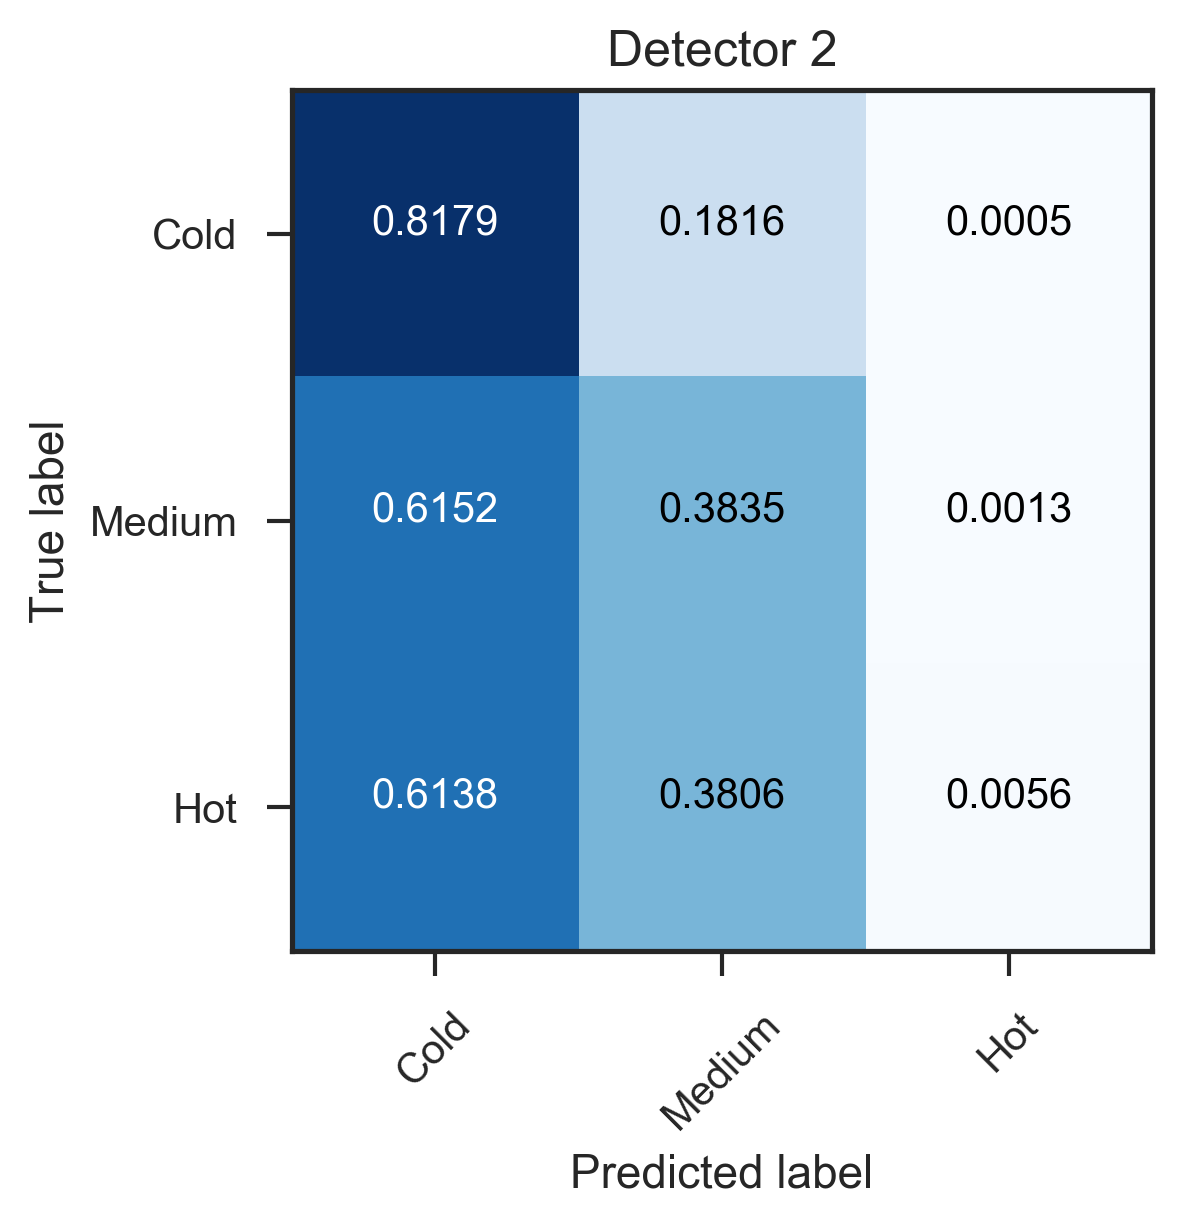
\includegraphics[width=0.45\textwidth]{drift_cm_Detector2.png}
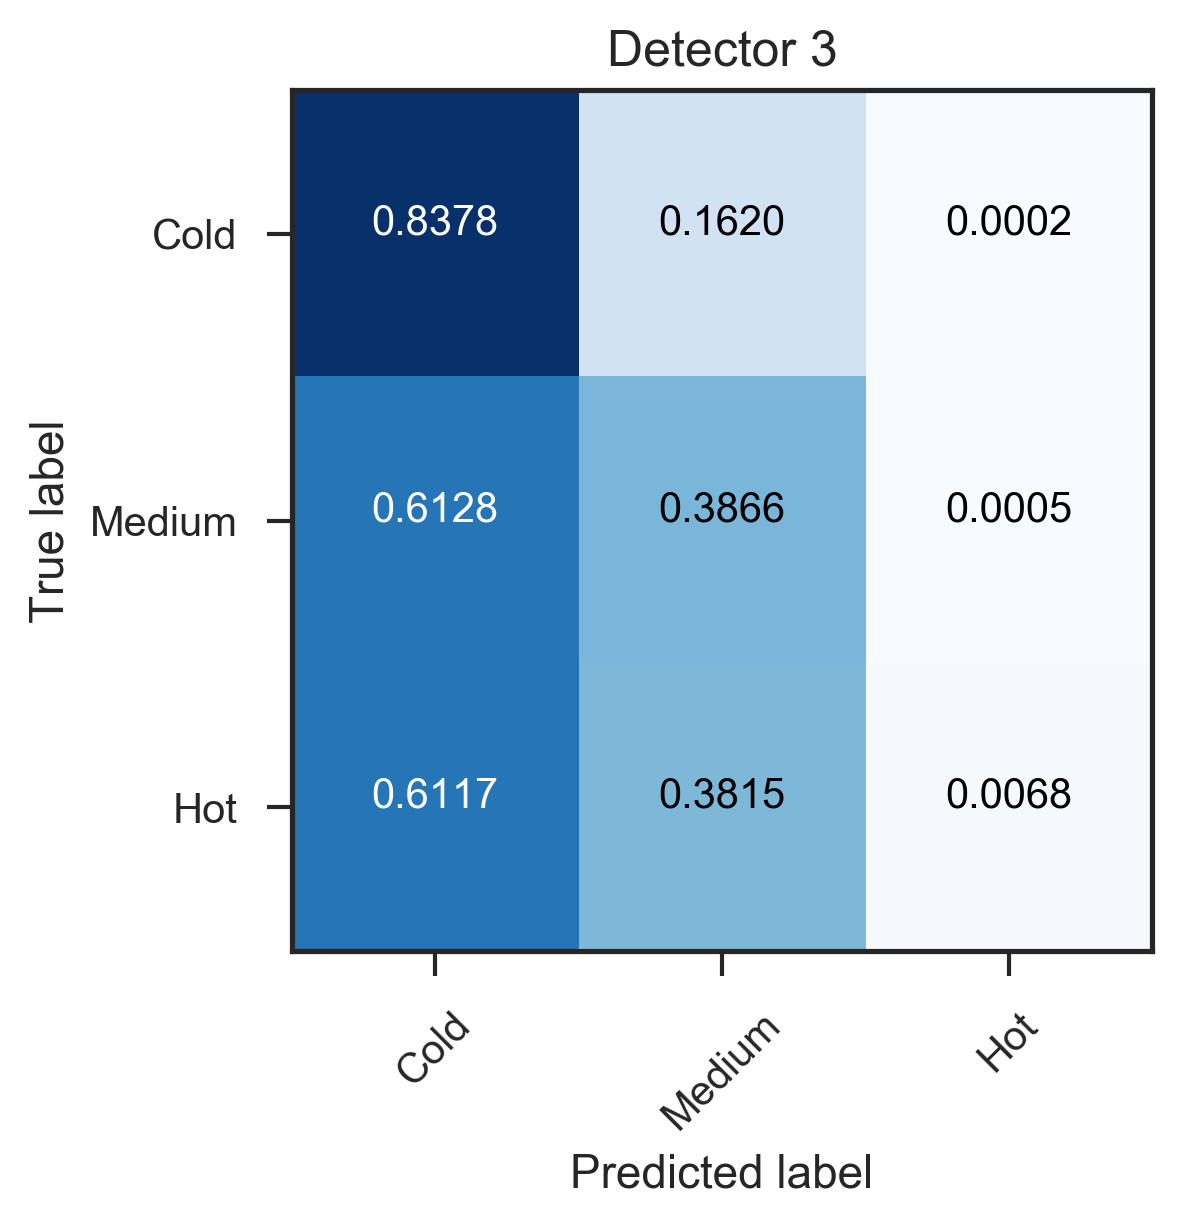
\includegraphics[width=0.45\textwidth]{drift_cm_Detector3.png}
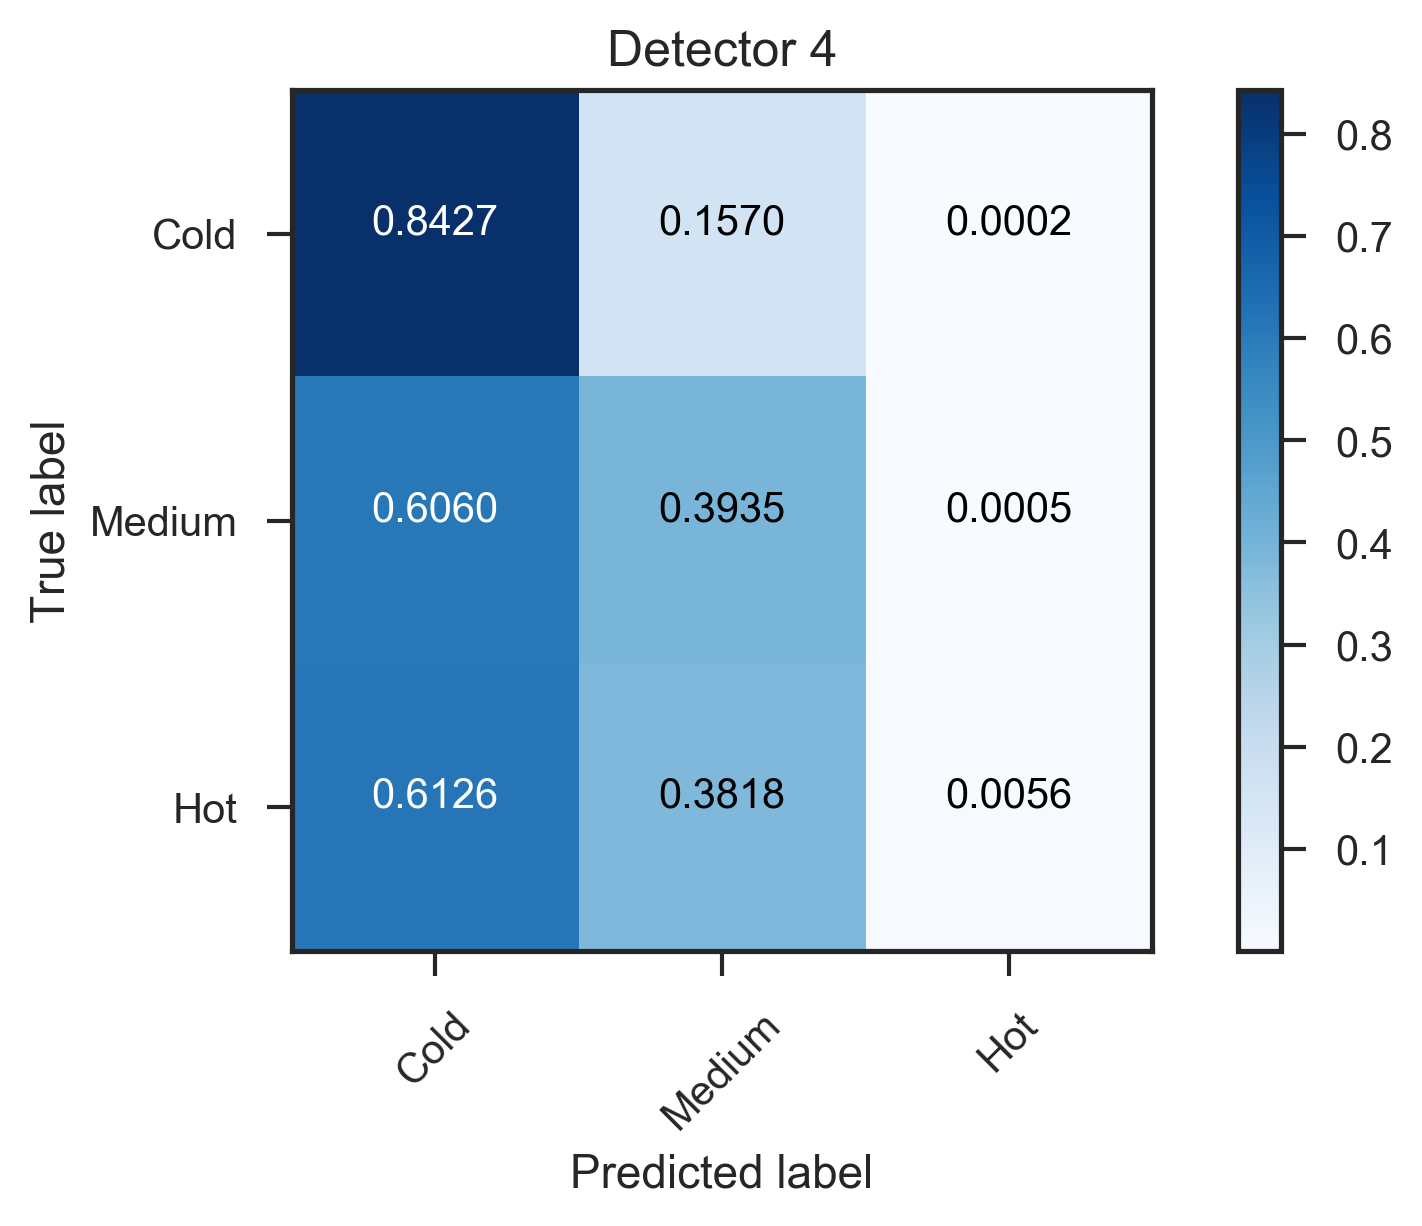
\includegraphics[width=0.45\textwidth]{drift_cm_Detector4.png}
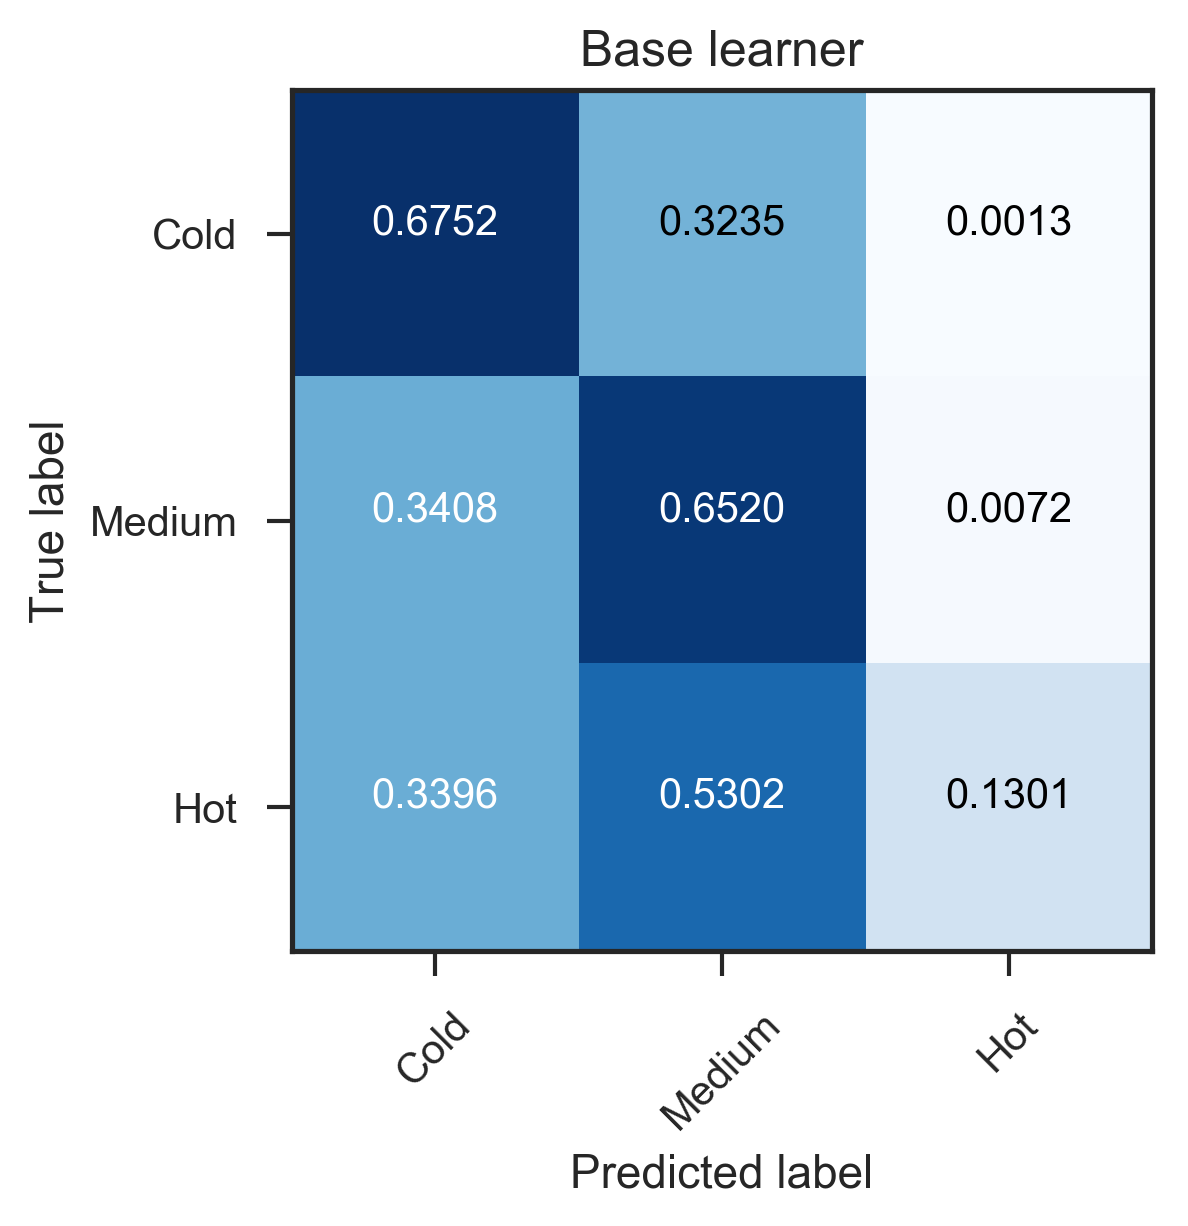
\includegraphics[width=0.45\textwidth]{drift_cm_Baselearner.png}
\caption{Confusion matrix of different detectors}
\label{drift_cm}
\end{figure}

\begin{figure}
\centering
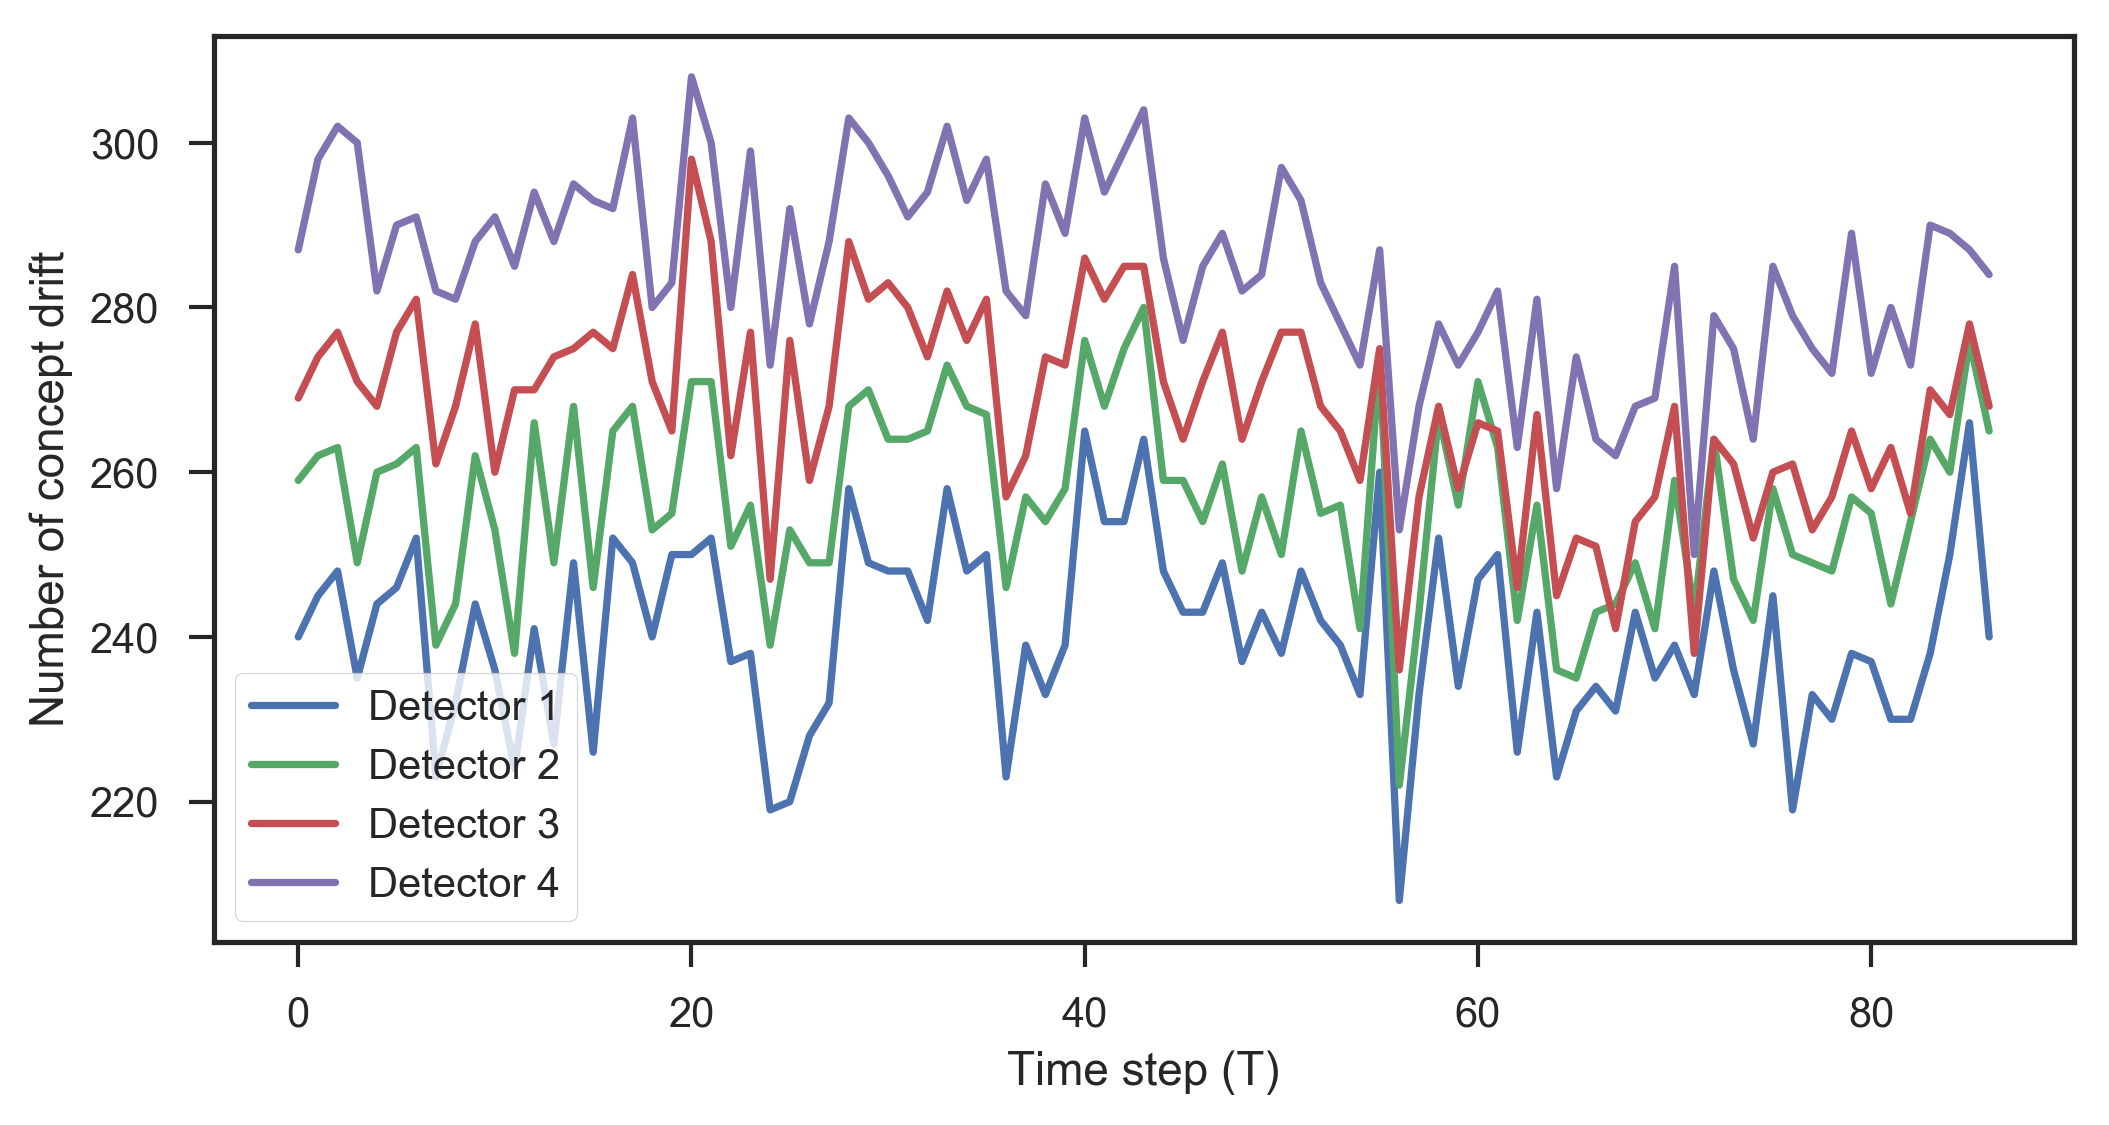
\includegraphics[width=0.9\textwidth]{num_cd.png}
\caption{Number of concept drift detected at each time step}
\label{num_cd}
\end{figure}

\begin{figure}
\centering
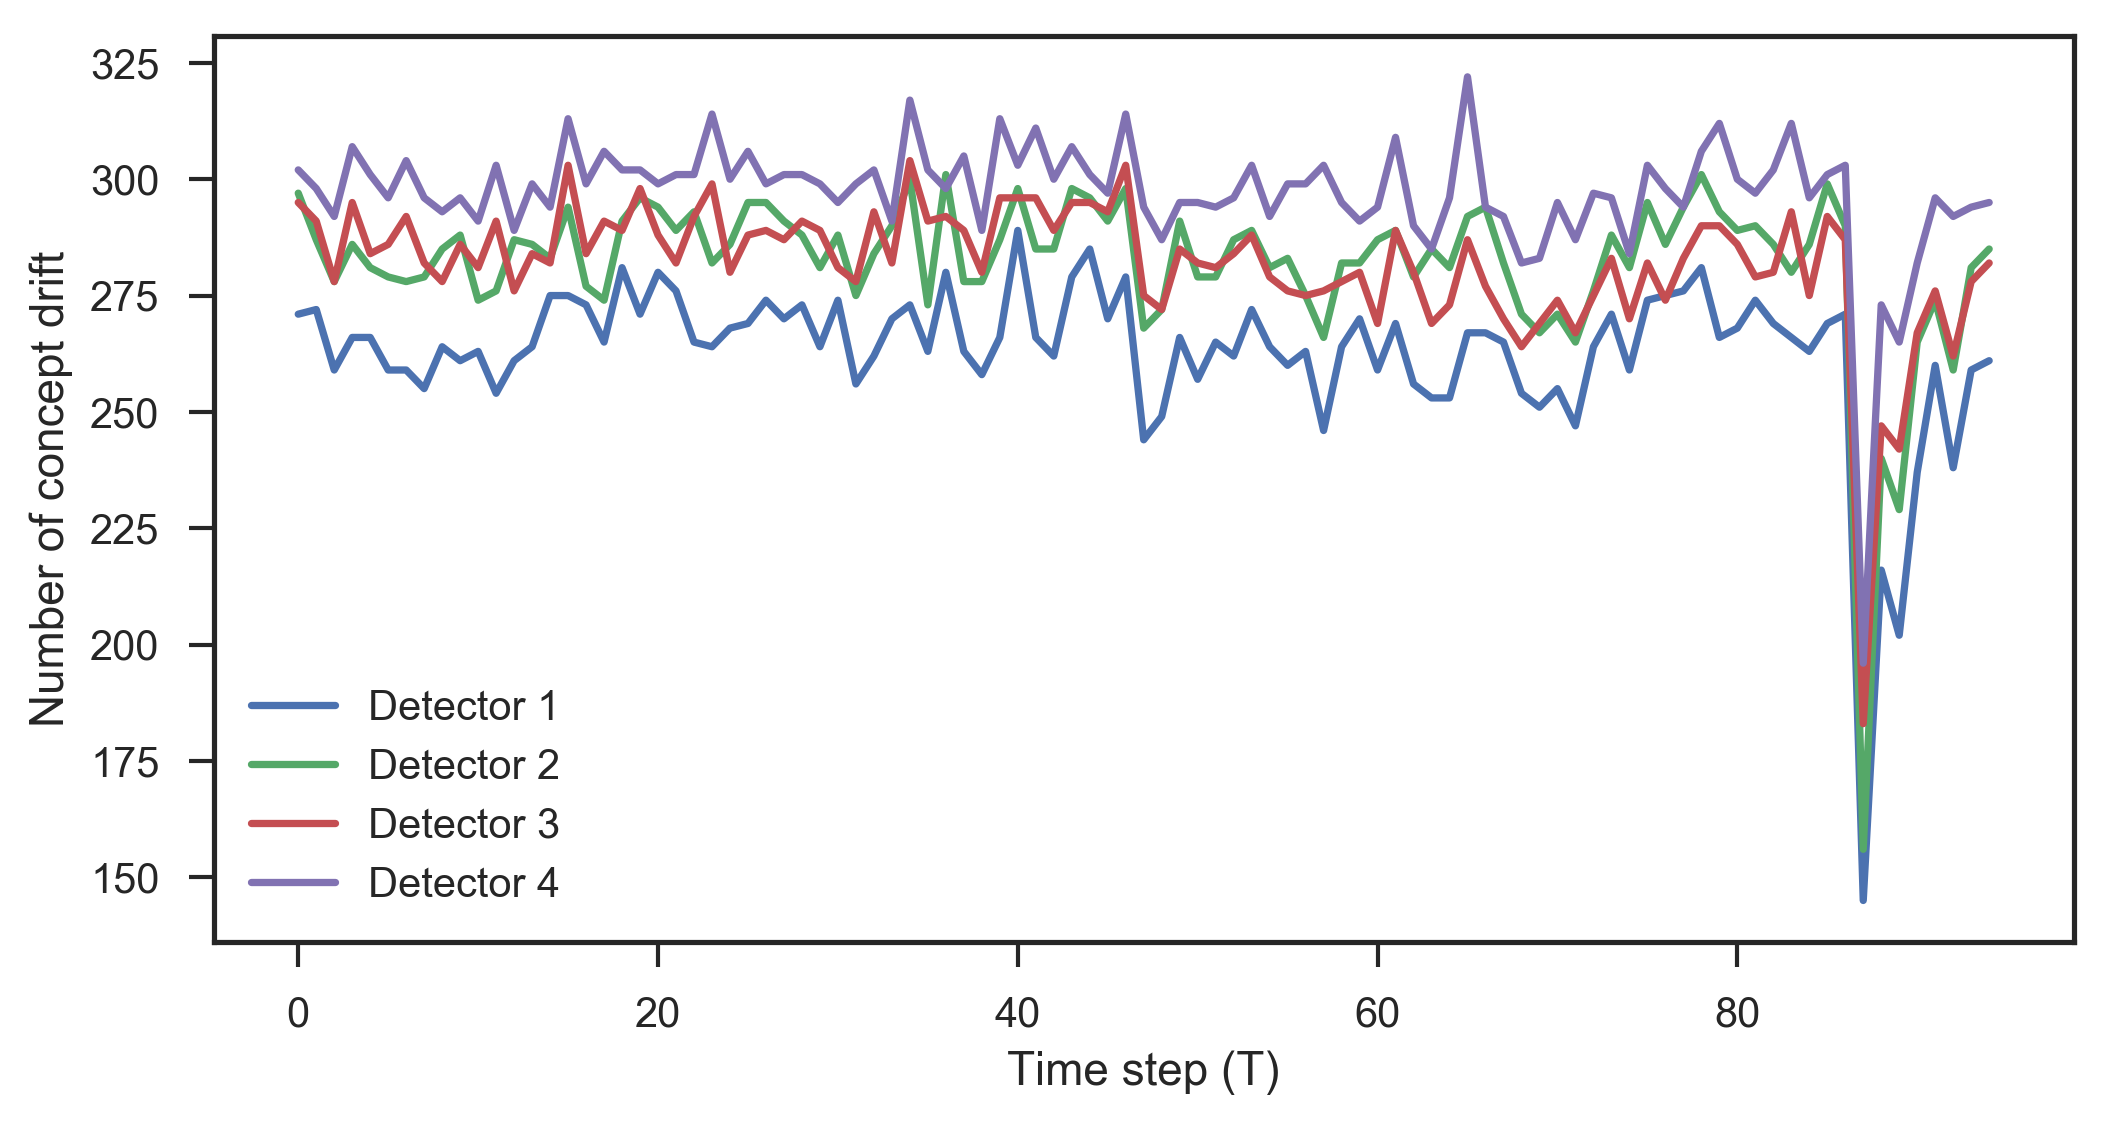
\includegraphics[width=0.9\textwidth]{num_fa.png}
\caption{Number of false alarm at each time step}
\label{num_fa}
\end{figure}


\begin{table}[]
\centering
\begin{tabular}{c|ccc}
Model       & Average & Recall & F1     \\ \hline
Detector 1  & 0.6018  & 0.4070 & 0.3921 \\
Detector 2  & 0.6011  & 0.4066 & 0.3918 \\
Detector 3  & 0.6128  & 0.4138 & 0.3985 \\
Detector 4  & 0.6130  & 0.4139 & 0.3986 \\ \hline
Base leaner & 0.6135  & 0.4357 & 0.4264
\end{tabular}
\caption{Averaged metrics of the detectors with different parameters}
\label{tabel_drift_metrics}
\end{table}

In this section, the results of the experiment with the drift detection framework, concerning the prediction performance and the drift detection ability, are presented.

Figure \ref{drift_metrics} shows graphics of accuracies, recalls, and F1 scores at each time step $T$ in the dataset. Each time step, there are $1000$ instance. Table \ref{tabel_drift_metrics} presents the averaged metrics of each detector and the base learner.

The confusion matrix


\subsection{Drift Identification}
\subsection{Predictive Accuracy}
\chapter{Multi-Input Deep Neural Network in Fashion News Popularity Prediction}
\label{exp2}

\begin{quote}
This chapter proposes a new deep learning model with two input layers to predict the fashion news popularity. The preprocessing of the deep learning model is introduced in detail. In addition, the techniques used in the model, including dropout, pooling, and bidirectional gate recurrent unit are discussed. This experiment further shows the prediction performance compared with four state-of-the-art model.
\end{quote}

\section{Data Used}
\label{dl_data}
In this experiment, we use similar dataset in experiment 1. The difference is that, as we do not use concept drift detection framework, we split the dataset into three parts. The fashion news from 1/04/2018 to 13/06/2018 are used as the test dataset. The dataset containing fashion news from 01/01/2014 to 31/03/2018 is split randomly into two subset. The subset containing 90\% news is used to training the model and the subset containing rest 10\% news is responsible to tune the hypeparameters. The number of examples in each dataset and the proportion of each class is shown in Table \ref{prop} 

\begin{table}[]
\centering
\begin{tabular}{c|cccl}
\multirow{2}{*}{Dataset} & \multirow{2}{*}{Number of news} & \multicolumn{3}{c}{Proportion of class} \\
                         &                                 & Hot         & Medium      & Cold        \\ \hline
Trian                    & 74996                           & 0.0721      & 0.3794      & 0.5485      \\
Validation               & 8333                            & 0.0728      & 0.3760      & 0.5512      \\
Test                     & 4188                            & 0.1445      & 0.3677      & 0.4878     
\end{tabular}
\caption{Properties of the datasets}
\label{prop}
\end{table}

To characterize the text classification problem and help tune the hypeparameters, the number of words in a sample from training set is collected and shown in Table \ref{num_words}


\begin{table}[]
\centering
\begin{tabular}{c|ccc}
\multirow{2}{*}{} & \multicolumn{3}{c}{Number of words per sample} \\
                  & Median        & Maximum        & Average       \\ \hline
Text              & 114           & 6258           & 158.59        \\
Title             & 19            & 59             & 19.60         \\
Keywords          & 3             & 36             & 3.24         
\end{tabular}
\caption{Number of words per sample}
\label{num_words}
\end{table}


\section{Model Design and Implementation}
This section introduces the preprocessing of the raw data which is shown in Figure \ref{dl_preprocess}. Then, the structure of the model is discussed. As shown in Figure \ref{dl_structure}, the model proposed in this section contains two parts. The first part receives the unigram and bigram of the keywords and title as the input. The architecture of this part is similar to fastText model which uses a word embedding layers that maps each word in the input into a low dimension word vector. Then, the word vectors is averaged to produce a sentence-level representation. The second part received the preprocessed text and also produce the word vectors by an embedding layer. The difference is that a bidirectional GRU is applied to model the word sequence and output the word-level representation. Then both a max pooling layer and an average pooling layer are used to merges the word-level representations. The sentence-level features are produced by concatenate the outputs from these two pooling layers. Finally, the prediction result is given by the fully connected layers.

The basic idea behind this model is that the order of the words and the long distance pattern is important for modeling the text but unimportant for modeling the titles and keywords. The word distribution is feature that we expect to extract from the keywords and titles. Thus, we design two different feature extractors, one inspired by fastTex focus on the word vectors and one similar to BLSTM~\cite{zhang2015relation} uses RNN component to extract the long distance pattern. These components will be discussed in detail in this section.


\subsection{Preprocessing}
\begin{figure}
\centering
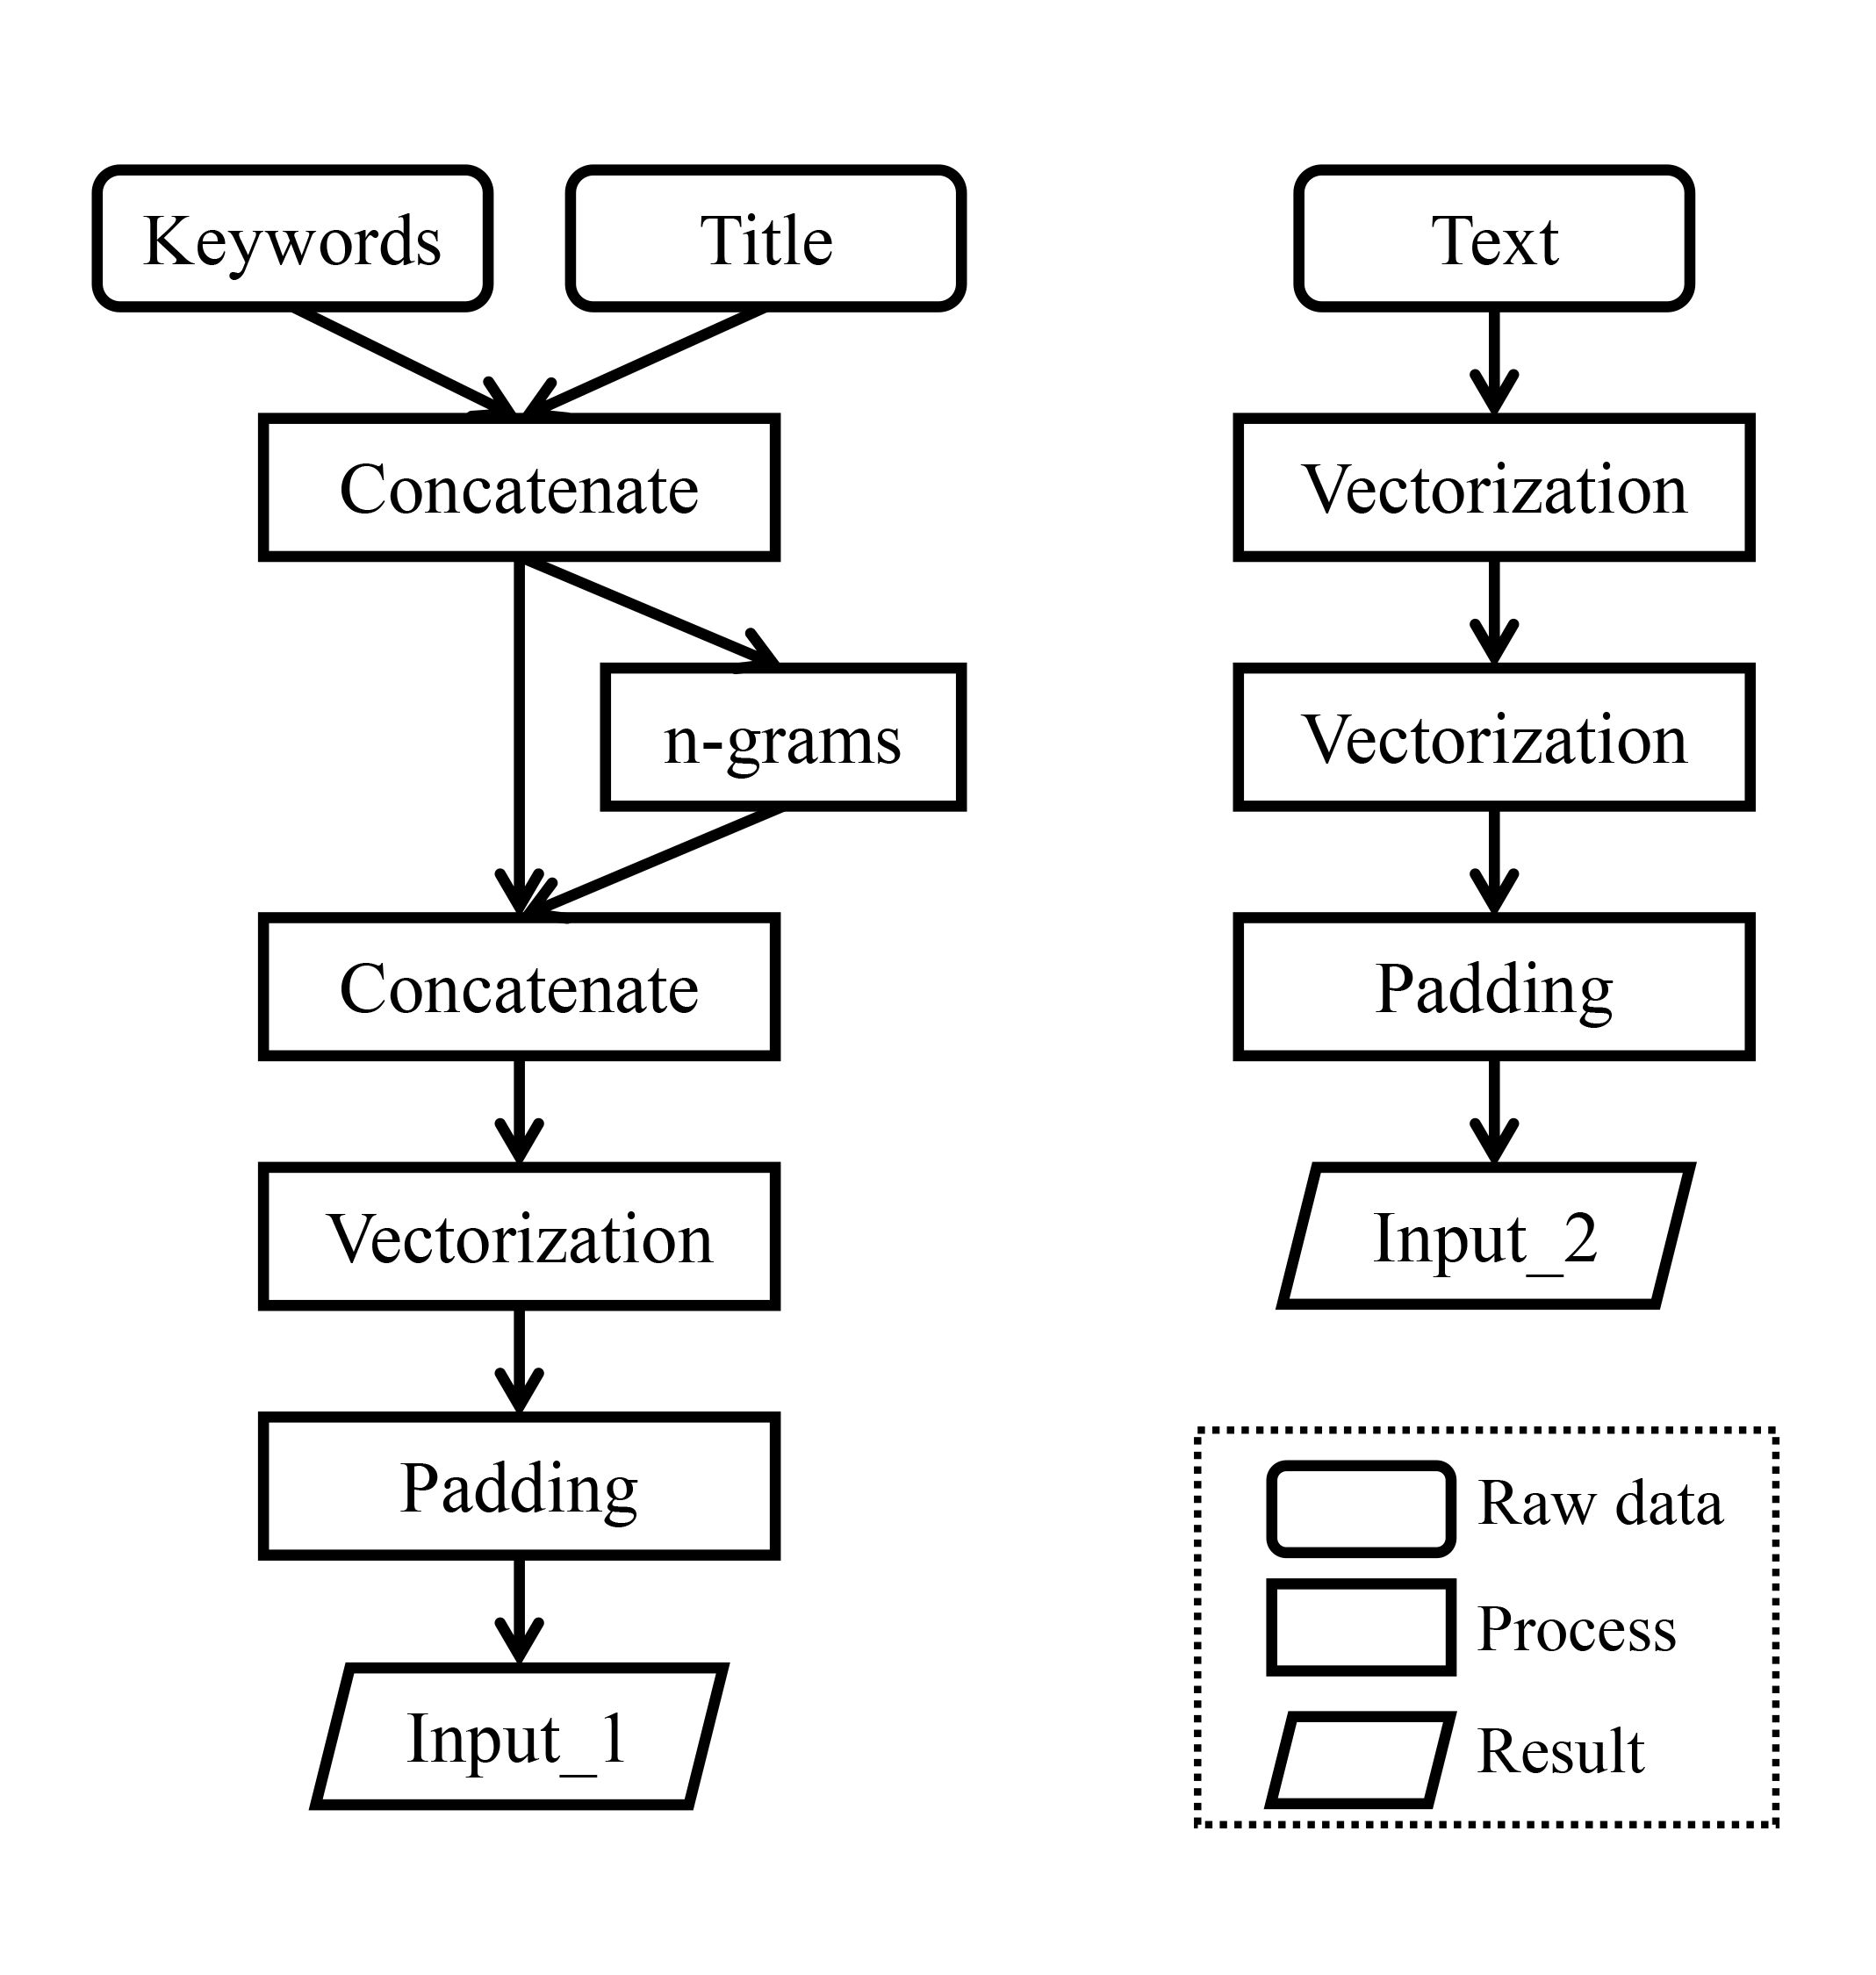
\includegraphics[width=0.6\textwidth]{dl_preprocess.png}
\caption{Preprocessing of the deep learning model}
\label{dl_preprocess}
\end{figure}

The procedure of the preprocessing for keywords, title, and text is shown in Figure \ref{dl_preprocess}. 

In a sample, the keywords and title are concatenate to a new sentence. Though the long distance pattern of this new sentence is not the one of the features we want, it is useful to capture some participial information about the local word order. Thus, the bag of n-grams is used as the additional feature. Considering the efficiency and most of keywords that are composed of two or fewer words, we use a bag of bigrams to keep the partial information. After this process, the sentence is represented as a sequence of unigrams and bigrams. Then the sequence is turned into numerical vector. A unique index is assigned to each unigram and bigrams. As keywords and title are the information extracted from the text, we keep all the words in our vocabulary.

However, not all words in the text contribute to the popularity predictions. In the process of tokening the text, the text is represented as a sequence of the unigrams and some rare and irrelevant words are discards from the vocabulary. In the experiment, we observe that using the most frequent 20,000 features is generally sufficient. 

The final step for two inputs is the padding. Sequences that are shorter than max length are padded with $0$ at the end while sequences longer than max length are truncated. In the experiment, the max length of the sequence is defined by the median number of words in each element. As shown in Table \ref{num_words}, the max length for title and keywords is sequence is $22$ and that for text is $114$.

\begin{figure}
\centering
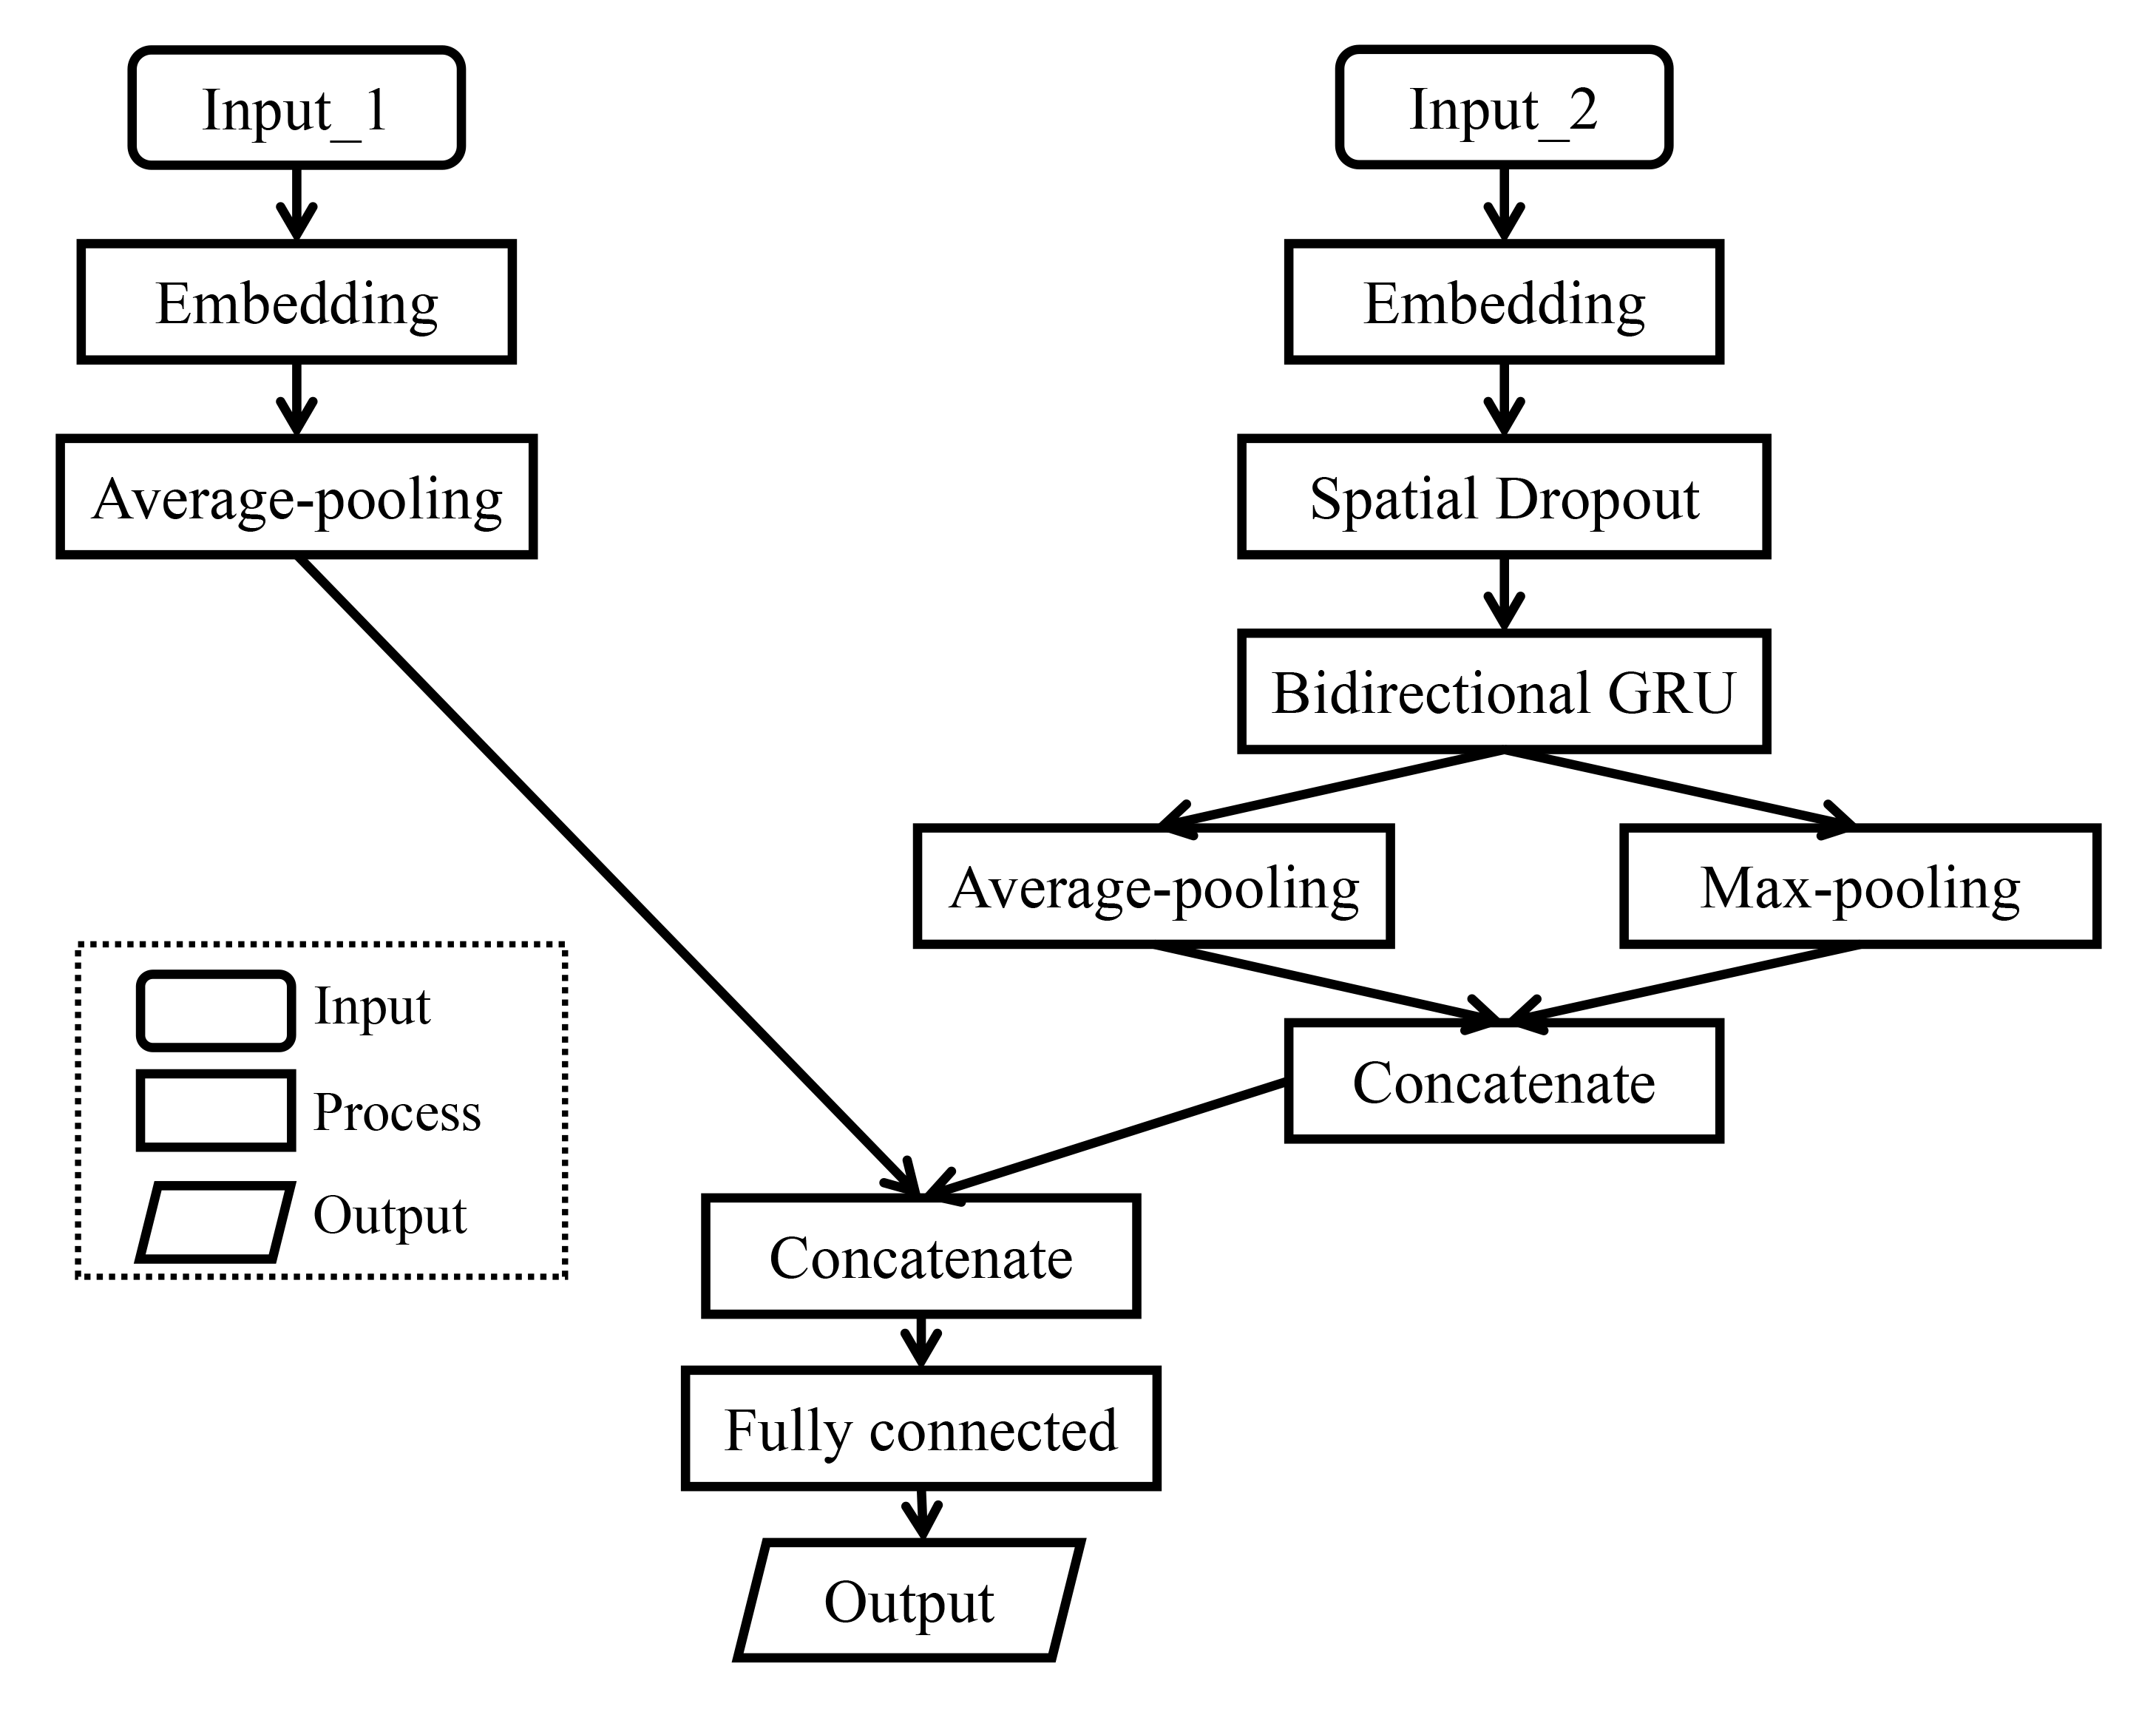
\includegraphics[width=0.8\textwidth]{dl_structure.png}
\caption{Structure of multi-input deep learning model}
\label{dl_structure}
\end{figure}
\subsection{Word Embeddings}
The first component of the proposed model is the word embedding layers. Both inputs are projected to low-dimensional word vectors by the embedding layers. After that, each word gets mapped to a dense vector of real values representing that word's location in semantic space. The advantage of using word vector is that the location and distance between vectors indicates how similar they are semantically. 

A sequence of $n$ indexes, where $n$ is the max length of the input which defined at the process of padding, is firstly transfered to one-hot encoding matrix $\mathbf{X}$. Let $\mathbf{X} \in \{1,0\}^{n \times V}$ where $V$ denotes the size of the vocabulary. The embedding layer transfers the one-hot encoding matrix into matrix containing composed of word vectors as follows
\begin{equation}
\mathbf{E} = \mathbf{X} \mathbf{W}
\end{equation}  

where $\mathbf{W} \in \mathbb{R}^{V\times D}$ and $D$ is the dimension of the word vector. Since $\mathbf{X}$ is one-hot, $\mathbf{W}$ is actually stores representations of all the words in the vocabulary.

There are two approach to initialize the projection weight $\mathbf{W}$. One is random initialization which will be updated during the training process. Another is using the pre-trained word vectors, by which the knowledge of general domains can be used. In our research, the embedding layer for the title and keywords is initialized randomly. Because, the keywords contains many celebrities' name, such as A\$AP Rockey, Young Nudy, and brands, such as YEEZY, Suicoke, which are not commonly used words so that the pre-trained word vectors do not contain these words. The dimension of the word vectors is set to $20$ as suggested by Joulin~\cite{Joulin2016}.

In contrast, the embedding layer for the text is initialized by the pre-trained weight. In order to compare with the work by Zhang~\cite{zhang2015relation} and Zhou et al.~\cite{zhou2016attention}, the model uses the same word vectors proposed by Turian et al. ~\cite{turian2010word}, which are 50-dimensional, to initialize the projection matrix.


\subsection{Bidirectional Gated Recurrent Unit Neural Networks}
\begin{figure}
\centering

\includegraphics[width=0.7\textwidth]{gru.png}
\caption{Graphical illustration of the GRU~\cite{Chung2014}.}
\label{GRU}
\end{figure}

The second component of the model is the bidirectional recurrent layer which is the key component for modeling the sequence and capture the long-distance pattern. 

We start from the gated recurrent unit(GRU). LSTM and GRU are both the variations of the RNN. But GRU can also be considered as a variation on the LSTM. The mechanism of the LSTM is introduced in Section \ref{background_lstm}. One of the difference between these two units is that GRU only has two gates which controls the information flow inside the units, however, without having an output gate that controls the exposure of the outputs. Another difference is the location of the input gate (reset gate). GRU controls the information from the previous activation when computing the new activation while LSTM controls it independently.

We assume $\mathbf{h}_t$ is the activation at time $t$ of the GRU, which is defined as follow
\begin{equation}
h_t^j = (1-z_t^j) h_{t-1}^j + z_t^j \hat{h}_t^j
\end{equation}
where $\mathbf{h}_{t-1}$ is the previous activation, $\hat{\mathbf{h}}_t$ is the candidate activation, and $\mathbf{z}_t$ is the update gate which controls how much of the past information needs to be passed along to the future. The update gate is computed by 
\begin{equation}
z_t^j = \sigma(W_z \mathbf{x}_t + U_z \mathbf{h}_{t-1})^j 
\end{equation}
In addition, the candidate activation $\hat{\mathbf{h}}_t$ is computed by the equation which is similar to the traditional recurrent unit. 
\begin{equation}
\hat{h}_t^j = \mbox{tanh}(W \mathbf{x}_t + U(\mathbf{r}_t \odot \mathbf{h}_{t-1}))^j
\end{equation}

where $\mathbf{r}_t$ is the reset gate which controls how much of past information flow to forget. Its computation is similar to the update gate 
\begin{equation}
r_t^j = \sigma(W_r \mathbf{x}_t + U_r \mathbf{h}_{t-1})^j
\end{equation}

As we discussed in Section \ref{background_lstm}, the problem of the one-directional forward RNN is that the information of the future vectors are not fully utilized. Thus, we use the bidirectional architecture to extract the features from both past words and future words. The graphic illustration of bidirectional LSTM is shown in Figure \ref{blstm}. The bidirectional GRU is same to bidirectional LSTM, just change the type of the unit. Zhang~\cite{zhang2015relation} and Zhou et al.~\cite{zhou2016attention} both summed the outputs from forward and backward. In order to retain as much information as possible, we concatenate the outputs from both directions. 

In the experiment, the  size of the GRU unit is set to 80. 

\subsection{Pooling Layer}
The third component of our model is the pooling layer. In the experiment, we use two types of pooling layers. The objective of using pooling layer is compress the word-level representations to sentence-level feature vectors. One of the compression method is the accumulation approach which use the feature vector produced at the last time step from RNN layer. However, we use the bidirectional RNN which can not defined what is last time step. Thus, most of RNN models resort to the pooling approach as in CNN models. 

However, different from the pooling layer used in CNN models which specify the kernel size of the pooling layer, the pooling layer in RNN are mostly the global pooling. In our research, the global max-pooling and global average-pooling are defined as follows:
\begin{equation}
m_i = \mbox{max}_t\{(h_t)_i\}
\end{equation}
\begin{equation}
m_i = \mbox{average}_t\{(h_t)_i\}
\end{equation}
where $m$ is the sentence-level feature vector and $i$ indexes features dimensions~\cite{zhou2016attention}. 

For title and keywords, we use the global average pooling which is suggested by ~\cite{Joulin2016}. For the text, the novelty is that we use two pooling methods and the sentence-level representation is produced by concatenating the outputs from the pooling layers. The hypothesis is that some keywords play important a role in prediction but the overview of the sentence is also very important. So max-pooling extracts the keywords information while average-pooling provides the overview of the sentence.


\subsection{Classifying}
The sentence-level feature vectors from title\&keywords and text are concatenated and passed to the final classifier. In the experiment, the fully connected neural network is classifier and softmax function is used to predict the label. For the concatenated feature vector $\mathbf{h}^* \in \mathbb{R}^{d}$, the prediction is given by
\begin{equation}
\mathbf{J} = W_j \mathbf{h}^* + b_j
\end{equation}
\begin{equation}
\hat(p)(y|S) = \mbox{softmax}(W_S \mathbf{J} + b_S)
\end{equation}
\begin{equation}
\hat{y} = \mbox{argmax}_y \hat{p}(y|S)
\end{equation}
where $W_j, b_j$ is the weights of the fully connected layer and $W_S, b_S$ is the weights of the output layer. 

As our dataset is very imbalance, traditional cost function, such as negative log-likelihood, does not punish the majority class. To solve this problem, we resort the focal loss in image classification. Focal loss was proposed by Lin et al. for dense object detection~\cite{Lin2017}. The definition of the focal loss can address the class imbalance by down-weighting the loss assigned to well-classified examples. 

We assume $t\in \mathbb{R}$ is the ground truth, $p_t$ is defined as 
\begin{equation}
p_t = \hat{p}(t|S)
\end{equation}

The focal loss is defined as 
\begin{equation}
\mbox{FL}(p_t) = -(1-p_t)^\gamma \mbox{log}(p_t)
\end{equation}

where $\gamma$ is the focusing parameter adjusting the rate at which easy examples are down-weighted. And when $\gamma = 0$, FL is equivalent to cross entropy. Focal loss shows its advantage when $p_t \rightarrow 1$. $(1-p_t)^\gamma$ goes to $0$ by which the easy example is down-weighted.


\subsection{Regularization}
We punish the complex model by adding an additional dropout layer after embedding layer. The role of dropout layer is preventing the activations from becoming strongly correlated so that the generalization of the model can be approved. It is an effective regularization method in deep learning model.

Instead of using standard dropout, we apply the spatial dropout to our model. The standard dropout set individual `pixel' to $0$randomly, which works well on images because adjacent pixels are highly correlated. However, the correlation between the feature vectors are more important on texts. Thus, Spatial dropout randomly omits the entire feature maps by setting them to $0$, which works better in our model~\cite{tompson2015efficient}.

In the experiment, the dropout rate is set to $0.2$, which indicates 20\% of the word vectors will be dropped.

\subsection{Evaluation Metrics}
The evaluation metrics in this experiment is similar to the experiment 1, including accuracy, macro-F1, macro-Recall, and the confusion matrix. The difference is that we use Area Under the macro averaged Receiver Operating Characteristic Curve (ROC AUC) score to evaluate the prediction performance.

A ROC curve is a graphical plot that illustrate the prediction ability of a binary classifier. The x-axis of the curve is the false positive rate (FPR) with different threshold. The FPR is defined as 
\begin{equation}
\mbox{FPR} = \frac{fp}{fp+tn}
\end{equation}
where $fp$ is number of positive instances which are incorrectly predicted, and $tn$ is the number of negative instances which are correctly predicted. The y-axis of the curve is the true positive rate (recall) with different threshold. 

ROC AUC score is obtained by computing the area under the ROC curve. ROC AUC store is 1 indicating perfect classifier and between 0 to 1 indicating the classifier is better than random guess. 

The definition of macro averaged ROC AUC score is same to macro-F1 and macro-Recall introduced in Section \ref{cd_metrics}, which calculates the metrics for each label and outputs the unweighted mean.

\subsection{Model Training}
The model is trained by training dataset and 
validated by the validation dataset, which described in Section \ref{dl_data}. The focal loss function is optimized by Adam optimization algorithm~\cite{Kingma2014}. Adam combines the advatanges of adaptive gradient algorithm (AdaGrad) and root mean square propagation (RMSProp) which can handle sparse gradients on noisy problem. In the training process, the Adam algorithm is applied with learning rate of 0.1 and mini batch size of 32.

To prevent overfitting and find the best model, the validation-based early stopping technique is used in the training process. 
At the end of each epoch, the ROC AUC score on validation dataset will be computed and the current weights of the model will be stored. In the experiment, the patience of the early stopping is set to $5$. After 5 epochs with no improvement of the ROC AUC score, the training will be stopped. The best model will be selected from the stored model with the highest ROC AUC score. 

In addition, except for the embedding layer for text inputs which is initialized with pre-trained word vectors, all the weights are initialized randomly. 

\subsection{Comparison Models}
Recently, a variety of the deep learning model have been applied to text classification. We choose four stat-of-the-art and representative models for comparison. These four models have different functional components and mechanisms which are discussed in Section \ref{dl}.

\textbf{fastText.} fastText only uses an embedding layer to extract word vectors and an global average pooling layer to produce sentence-level representation. It is a fast and effective classification model which widely used as a baseline model. The parameters of used in comparison is same to the model described in the original paper ~\cite{Joulin2016}. The embedding layer is initialized randomly and the dimension of the word vector is set to $20$. The inputs the sequence concatenating the title and text.

\textbf{Character-level Convolutional Network}
The char-level CNN is only one comparison model whose functional layer is the convolutional layer. The advantage of the char-level CNN is that it has very high fault tolerance. As it classify the text in character level, it can easily deal with the typos or the unseen words. The model structure used in comparison is same to what is described in Table \ref{config_char_cnn} and Table \ref{config_char_fl}. We use the same low-case alphabet presented in Section \ref{cnn_background}.

\textbf{Bidirectional Long-Short Term Memory Network.}
The BLSTM used in comparison is the model introduced in Section \ref{background_lstm}. The size of LSTM unit is set to $256$ as suggested by the author. To ensure fair comparison, the embedding layer is initialized with the same pre-trained word vectors proposed by Turian et al. ~\cite{turian2010word}. The model is trained by stochastic gradient descent algorithm. 

\textbf{Attention Based Bidirectional Long Short-Term Memory Network.}
The Att-BLSTM has same bidirectional RNN layer with BLSTM. In addition, its embedding layer is also initialized with the Turian's pre-trained weights. The difference is that Att-BLSTM is trained by AdaDelta and regularized the model parameters with L2 regularization strength of $10^{-5}$.



\section{Experimental Results}

%\chapter{Stock Price Movement Prediction Model}
\label{chapter1}
\section{Background}
\subsection{Motivation}
\subsection{Related Work}
\subsection{Statistical Analysis}
\section{Experiment}
\subsection{Dataset}
\subsection{Model Design}
\subsection{Results}

\chapter{Conclusions and Future work}
\label{conclusion}
\section{Summary of Contributions}
\section{Future Work}

% This just dumps some pseudolatin in so you can see some text in place.
\blindtext

%\addcontentsline{toc}{chapter}{Appendices}

% The \appendix command resets the chapter counter, and changes the chapter numbering scheme to capital letters.
%\chapter{Appendices}
\appendix
\chapter{An Appendix About Stuff}
\label{appendixlabel1}
(stuff)

\chapter{Another Appendix About Things}
\label{appendixlabel2}
(things)

\chapter{Colophon}
\label{appendixlabel3}
\textit{This is a description of the tools you used to make your thesis. It helps people make future documents, reminds you, and looks good.}

\textit{(example)} This document was set in the Times Roman typeface using \LaTeX\ and Bib\TeX , composed with a text editor. 
 % description of document, e.g. type faces, TeX used, TeXmaker, packages and things used for figures. Like a computational details section.
% e.g. http://tex.stackexchange.com/questions/63468/what-is-best-way-to-mention-that-a-document-has-been-typeset-with-tex#63503

% Side note:
%http://tex.stackexchange.com/questions/1319/showcase-of-beautiful-typography-done-in-tex-friends 
% You could separate these out into different files if you have
%  particularly large appendices.

% This line manually adds the Bibliography to the table of contents.
% The fact that \include is the last thing before this ensures that it
% is on a clear page, and adding it like this means that it doesn't
% get a chapter or appendix number.
\addcontentsline{toc}{chapter}{Bibliography}

% Actually generates your bibliography.
\bibliography{reference}

% All done. \o/
\end{document}
